% Fonte tam 12, papel A4, páginas do sumário não tem numeração
\documentclass[12pt, a4paper, tocpage=plain]{abnt}

\usepackage[brazilian]{babel} % Nomes e datas português com estilo brasileiro
\usepackage{hyperref} % cria hyperlink
\hypersetup{
  colorlinks=true, % false: caixa; true: apenas colore
  linkcolor=black, % cor do link
  citecolor=black, % cor dos link em bibliografia
  urlcolor=blue
}
\usepackage[utf8]{inputenc} % Suporte à caracteres especiais (acentos e cedilha)
\usepackage[T1]{fontenc}
\usepackage[alf]{abntcite} % Estilo de referência bibliográfica
\usepackage{graphicx} % Permite a utilização de imagens no documento
\usepackage[table,xcdraw]{xcolor} % Permite colorir tabela
\usepackage{longtable} % Permite utilizar tabelas grandes que ocupam mais paginas
\usepackage[small]{caption} % Define legendas das figuras com fontes menores
\usepackage{pslatex} % Define que o formato da letra será Times New Roman
\usepackage{epigraph} % Permite a criação de epígrafes
\usepackage{setspace} % Permite a definição de espaçamento entre linhas
\usepackage{nomencl} % define nomeclaturas para listas de siglas
\usepackage{listings}
\usepackage{color}
% Define as margens da folha
\usepackage[top=3cm, left=3cm, right=2cm, bottom=2cm]{geometry}

\setcounter{secnumdepth}{3} % Até três subsubsections numeradas
\setcounter{tocdepth}{3} % Até trẽs subsubsections numeradas
\setlength{\parindent}{1.25cm} % Recuo da primeira linha dos parágrafos (1.25cm)

\renewcommand{\ABNTchapterfont}{\bfseries} % Fonte do \chapter
\renewcommand{\ABNTchaptersize}{\large} % Tamanho da fonte \chapter
\renewcommand{\ABNTsectionfontsize}{\large} % Tamanho da fonte \section
\renewcommand{\ABNTsubsectionfontsize}{\large} % Tamanho da fonte \subsection
\renewcommand{\ABNTsubsubsectionfontsize}{\large} % Tamanho da fonte \subsubsection
% Título das referencias \bibliographys
\renewcommand{\ABNTbibliographyname}{REFERÊNCIAS BIBLIOGRÁFICAS}
\citeoption{abnt-repeated-author-omit=yes}
\bibliographystyle{abnt-alf}

\begin{document} % Começo do Projeto
\begin{titlepage}
 \begin{center}
   {\large UMA PERSPECTIVA REGIONAL DO GERENCIAMENTO DE PROJETOS EM UM POLO DE INOVAÇÃO} \\ [7cm]
   {\large PRISCILA MANHÃES DA SILVA} \\ [4cm]
   \vfill
   {\large UNIVERSIDADE ESTADUAL DO NORTE FLUMINENSE – UENF} \\ [1.5cm]
   {\large CAMPOS DOS GOYTACAZES – RJ} \\
   {\large JULHO – 2016}
 \end{center}
\end{titlepage}
 % Cria a capa
\newpage\null\thispagestyle{empty}\newpage % pagina em branco
\begin{titlepage}
 \begin{figure}[ht]
 \centering
 \scalebox{0.35}{\includegraphics{figuras/logo}}
 \end{figure}
 \begin{center}
   {\large BACHAREL EM SISTEMAS DE INFORMAÇÃO} \\ [3.5cm]
   {\large PRISCILA MANHÃES DA SILVA} \\ [4cm]
   {\large DESENVOLVIMENTO DE NOVAS FUNCIONALIDADES PARA A FERRAMENTA DE MANIPULAÇÃO DE ARQUIVOS EM NUVEM}\\ [2cm]
   \hspace{.45\textwidth} % posicionando a minipage
   \begin{minipage}{0.5\textwidth}
   \begin{espacosimples}
        Trabalho de conclusão de curso apresentado ao Instituto Federal Fluminense como requisito obrigatório para obtenção de grau em Bacharel de Sistemas de Informação.\\[1.5cm]
        Orientador: Prof. Rogério Atem Carvalho\\
        Co-orientador: Prof. Fernando Carvalho
    \end{espacosimples}
    \end{minipage}
   \vfill
   {\large Campos dos Goytacazes/RJ} \\
   {\large 2012}
 \end{center}
\end{titlepage}
 % Cria a folha de rosto
\begin{folhadeaprovacao}
    \setlength{\ABNTsignthickness}{0.4pt}
    \setlength{\ABNTsignwidth}{15cm}
    \setlength{\ABNTsignskip}{0.9cm}
    \begin{center}
       {\large UMA AVALIAÇÃO DO IMPACTO INICIAL DO USO DE FERRAMENTAS DE GESTÃO DE PROJETOS EM UM POLO DE INOVAÇÃO} \\ [3.5cm]
       {\large PRISCILA MANHÃES DA SILVA} \\ [1.5cm]
        \hspace{.45\textwidth} % posicionando a minipage
        \begin{minipage}{0.5\textwidth}
        \begin{espacosimples}
        Projeto para dissertação submetido à Universidade Estadual do Norte Fluminense Darcy Ribeiro, como parte das exigências para obtenção do título de Mestre em Engenharia de Produção.
        \end{espacosimples}
        \end{minipage}
    \end{center}
    {\normalsize Aprovada em \underline{\hspace{.2in}} de \underline{\hspace{.8in}} de 2016} \\\\
    {\normalsize Comissão Examinadora: }
    \bigbreak
    \assinatura{Prof. \underline{\hspace{10cm}} (Doutor(a), \\ \underline{\hspace{10cm}} ) - UENF}
    \bigbreak
    \assinatura{Prof. Simone Vasconcelos Silva (Doutora, Computação) - IFF \\ Coorientadora}
    \bigbreak
    \assinatura{Prof. Rogério Atem Carvalho (Doutor, Ciências de Engenharia) - IFF/UENF \\ Orientador}
\end{folhadeaprovacao}
 % Cria a folha de aprovação
% \null
\vfill

{\normalsize \it \hfill Dedico este trabalho à minha mãe e amigos por todo apoio, compreensão \vspace*{4pt}

\hfill e contribuição que me prestaram.}  % Cria a folha de dedicatória
% \begin{center}
\textbf{AGRADECIMENTOS}
\end{center}

Primeiramente agradeço a minha mãe que sempre esteve ao meu lado nestes longos anos.
Agradeço também a todos meus amigos e colegas de trabalho do NSI, que me apoiaram e incentivaram.
Bem como aos professores Rogério Atem e Fernando Carvalho que contribuiram muito para que esse projeto fosse realizado.
 % Cria a folha de agradecimentos
% \null % o \vfill só funciona com o \null
\vfill
\epigraph{O computador não é mais o centro do mundo digital.}{Tim Cook} % Cria a epígrafe
% \begin{center}
\textbf{RESUMO}
\end{center}
\singlespacing

\noindent . \\

\noindent Palavras-chave:
 % Resumo do trabalho
% \begin{center}
\textbf{ABSTRACT}
\end{center}

\singlespacing

\noindent This work describes about the development of new functionalities to a free tool of document manipulation on a large scale, being this new functionalities responsible for allowing the tool to adapt in handling other file formats, such as multimedia ones, for example. It stills describes a little about the applications and/or other tools used for integrating its own with propose to handle with this new functionalities. Through this partnership between the French company Nexedi SA with the aid of the Nucleus of Research in Information Systems (NSI-IFF), was possible to implement the ability to manipulate shapes corresponding to video files, audio, images and PDF; being this manipulate as well responsible for converting, inserting and extracting data from this files. Still can find in this job, the structure of this tool, basic concepts used to create the tool and integrate it with the core Linux, as well as concepts of Python, which was used for its development. \\

\noindent KEYWORDS: Web Service, Free software ,Python, Cloud Computing 

 % Resumo em língua estrangeira

\singlespacing % espaço simples
\renewcommand{\listfigurename}{LISTA DE FIGURAS} %Nome para lista de figuras
\listoffigures % Gera o índice de figuras
\renewcommand{\listtablename}{LISTA DE TABELAS} % Nome para lista de tabelas
\listoftables % Gera o índice de tabelas
\makenomenclature % cria lista de siglas (makeindex tcc.nlo -s nomencl.ist -o tcc.nls)
\renewcommand{\nomname}{LISTA DE SIGLAS} % Nome para lista de siglas
\printnomenclature % Gera o índice de siglas
\renewcommand{\contentsname}{SUMÁRIO} % Nome do sumário
\tableofcontents % Gera o sumário

\onehalfspacing % Espaçamento de 1.5cm entre linhas
% Capitulos variam de acordo com o projeto, um arquivo para cada
\nomenclature{APM}{Agile Project Management}
\nomenclature{CT\&I}{Ciência, Tecnologia e Inovação}
\nomenclature{GP}{Gestão de Projetos}
\nomenclature{GAP}{Gestão Ágil de Projetos} % ???
\nomenclature{GPP}{Gestão de Portfólio de Projetos}
\nomenclature{EP}{Escritório de Projetos}
\nomenclature{EMBRAPII}{Empresa Brasileira de Inovação Industrial}
\nomenclature{PMBOK}{\textit{Project Management Body of Knowledge} (Conjunto de conhecimentos em gerenciamento de projetos)}
\nomenclature{PMI}{\textit{Project Management Institute} (Instituto de Gerenciamento de Projetos)}
\nomenclature{PMO}{\textit{Project Management Office} (Escritório de Projetos)}
\nomenclature{PMP}{\textit{Project Management Profissional} (Profissional de Gerenciamento de Projetos)} % ???
\nomenclature{PMI-ACP}{\textit{PMI Agile Certified Practitioner Profissional} (Profissional Certificado em Métodos Ágeis do PMI)} % ???
\nomenclature{PI}{Polo de Inovação}
\nomenclature{PICG}{Polo de Inovação Campos dos Goytacazes}
\nomenclature{P\&D}{Pesquisa e Desenvolvimento} % ???
\nomenclature{P\&DI}{Pesquisa, Desenvolvimento e Inovação} % ???
\nomenclature{SI}{Sistemas de Inovação}
\nomenclature{SNI}{Sistema Nacional de Inovação} % ???
\nomenclature{TI}{Tecnologia de Informação}
 % separando siglas em um arquivo
\chapter{INTRODUÇÃO}
\thispagestyle{empty}

\section{Contextualização}
  Quando custo e qualidade deixaram de ser a principal motivação de melhoria nas organização, e a importância dos processos inovação como meio de distinção de produto e manutenção da competitividade foi salientada junto a necessidade do atendimento às constantes modificações de requisitos por parte dos clientes, que se destacaram ainda mais como alvo das organizações \cite{atkinson2012global}.

  Para os autores \citeonline{prado2006mmgp, pmiguide2013}, apenas por meio da realização de projetos que empresas se tornam capazes de realizar as mudanças necessárias e atender às crescentes exigências dos consumidores por obter produtos, ou serviços, de excelência, dentro do prazo e custo estabelecidos adequadamente.

  É possível notar que nos últimos anos, tanto em organizações privadas quanto públicas, existe uma necessidade de estabelecer melhores ações estratégicas que sejam capazes de responder de forma àgil e eficaz as mudanças propostas nos projetos, porém que não concluam na insatifação dos resultados desses projetos \cite{de2008construindo}.

  Frente a problemática da satisfação do cliente com as entregas efetuadas pelos projetos, e procurando viabilizar ferramentas, técnicas e soluções para a gestão de projetos (GP), alguns autores buscaram apresentar processos que representam melhores que práticas e que por vezes incluem modelos de maturidade como meio de vincular a melhoria na performance dos projetos a evolução de uma escala de aderência às práticas recomendadas \cite{kerzner2013project, pmiguide2013, prado2006mmgp}.

  Entretanto, \citeonline{atkinson2012global} demonstraram uma certa preocupação de que essas abordagens se envolvessem mais com a eficiência do projeto, do que com o atendimento às expectativas dos participantes envolvidos na criação deles, entre os quais o cliente mais uma vez se destaca.

  A estrutura de gerenciamento chamada de escritório de gestão de projetos (EGP) passou a se destacar por representar uma padronização dos processos de governança relacionados ao projetos que visam o compartilhamento de recursos, metodologias, ferramentas e técnicas. Assim, essa estrutura pode ser responsável por um ou mais projetos, auxiliando-os a alcançar seus objetivos com excelência, de acordo com seus requisitos e aumentando a taxa de sucesso \cite{pmiguide2013}.

  Em outro ponto, \citeonline{garnica2009gestao} demonstrou preocupação quanto a gestão de projetos em nível tecnólogico no contexto das instituições de ensino, que vêm se destacando como meio de conectar atividades de pesquisa a utilização de novos conhecimentos para a sociedade, provendo assim fontes de inovação.

  Esse aumento da dependência da inovação, advinda do meio da pesquisa, como principal fator de crescimento econômico traz a necessidade de uma forma de controle as regras de crescimento e a coordenação dos Sistemas de Inovação (SI) que tendem a surgir para promover a sustentabilidade e competitividade a longo prazo \cite{lundvall2010politicas}.

  No Brasil, a Associação Brasileira de Pesquisa e Inovação Industrial (EMBRAPII), se destaca por promover a união igualitária de responsabilidade de financiamento de dois importantes orgãos federais, o Ministério da Ciência, Tecnologias, Inovações e Comunicações (MCTIC) e o Ministério da Educação (MEC). Além deste envolvimento, em recente comunicado a associação anunciou a parceria com o Instituto Federal Fluminense (IFF), para formação do Polo de Inovação Campos dos Goytacazes (PICG), e salientou sua missão de contribuir para o desenvolvimento da inovação na industria através da pesquisa.

  Para averiguar a efetividade dos processos de gestão de projetos, dentro de um escritório de gestão de projetos do Polo de Inovação, este trabalho pretende apresentar uma revisão da literatura no quesito da gestão de projetos, e o contexto para a implementação do mapeamento da maturidade desses projetos frente ao modelo EMBRAPII.

% \section{Problemática}

% o modelo EMBRAPII foi desenvolvido levando em consideração experiência passada mas se conferir se, ou sem ser comparado com um modelo conhecido e abrangido internacionalmente, como o CMMI

\section{Objetivos}

  Para que haja melhor compreensão do trabalho, os obejtivos encontram-se divididos em objetivo geral e objetivos específicos.

  \subsection{Objetivo Geral}
  % O objetivo deste trabalho é avaliar se a evolução na maturidade em gerenciamento de projetos conduz a melhorias no gerenciamento e, consequentemente, no nível de desempenho dos projetos, bem como identificar as principais dificuldades encontradas neste processo de evolução

  Verificar através de um mapeamento e de um estudo de caso se os conceitos e ferramentas empregados na gestão de projetos dentro de um escritório de projetos, podem efetivamente contribuir na busca por inovação e competitividade do mercado.


  \subsection{Objetivos específicos}

  \begin{itemize}
    \item{Levantar literatura científica sobre o tema;}
    \item{Observar em campo a aplicação de abordagens de gestão de projetos em um escritório de projetos;}
    \item{Analisar e discutir sobre o uso dessas abordagens;}
    \item{Avaliar a diferença de produtividade implícita no escritório de projetos;}
    \item{Verificar a adequação da mesclagem de práticas tradicionais e agéis da gestão de projetos;}
    \item{Verificar a adequação do Polo de Inovação Campos dos Goytacazes (PICG) frente ao plano de ação da EMBRAPII.}
  \end{itemize}


\section{Justificativa}

  Este trabalho apresenta uma visão sobre abordagens de gestão de projetos, referenciando também a gestão de programas e portfólio, bem como seu enquadramento nos escritórios de gestão de projetos. Apresenta-se também o objeto de caso de estudo, o PICG, um polo de inovação com recente implantação de um escritório de projetos, que se aproxima de sua primeira entrega.

  A contribuição almejada neste trabalho será o mapeamento de um modelo de maturidade de projetos, imposto pela EMBRAPII, para contribuir com a representação da efetividade da GP neste ambiente.

\section{Estrutura do trabalho}

  Este projeto está organizado em quatro capítulos, um apendíce e um anexo. No primeiro capítulo foi apresentado o contexto no qual a pesquisa se encaixa frente as motivações do trabalho e seus objetivos.

  O segundo capítulo apresentada uma revisão bibliográfica no que respeito as práticas de gestão de projeto, relacionando seus conceitos, motivações e situação atual.

  O terceiro capítulo propõe a metodologia que será empregada no trabalho, destacando sua natureza, sua população e amostragem, frente ao objeto do estudo de caso, o PICG.

  O ultimo capítulo representa um espaço para discussão dos resultados a serem obtidos nesta pesquisa, com as considerações finais e um cronograma de execução do projeto.

  No apendíce encontra-se uma análise bibliográfica sobre o tema, e inclui uma apresentação dos periódicos escolhidos para esse projeto.

  O anexo representa o artigo desenvolvido, a partir de uma revisão bibliográfica de temática às práticas de gestão de projetos ao longo dos anos, para cumprimento das exigências a apresentação deste projeto.
 % Capitulo 1
\chapter{REVISÃO DA LITERATURA}
\thispagestyle{empty}

\section{Projetos}

\citeonline[p. 8]{meredith2011project} definem que projetos tratam da realização de tarefas específicas e finitas, de grande ou pequena escala, com um prazo de execução e um orçamento estipulado. \citeonline{turner2014handbook}, por sua vez, dispõe que projetos são tarefas com uma data final, onde caso esta data não implique na entrega do projeto, será estabelecida uma entrega do produto presente e a criação de outro projeto para entregar as tarefas restantes, referente a este produto.

Para \citeonline{kerzner2013project} um projeto pode ser caracterizado por uma série de atividades e tarefas realizadas com um objetivo específico para serem completadas sob determinadas especificações. Essas atividades e tarefas também devem possuir datas definida para inicio e fim; limites de recursos e custos; bem como um quantitativo de pessoas e equipamentos que será envolvido nestas.

Finalmente, de acordo com o \citeonline{pmiguide2014}, um projeto pode ser compreendido por um esforço temporário empreendido a fim de criar um produto, prestar serviço ou trazer um resultado exclusivo. Esse esforço é composto por um conjunto de atividades inter relacionadas e direcionadas à obtenção de um ou mais produtos únicos, com tempo e custos definidos. Nesta definição, algumas características básicas do projeto devem ser destacadas:

\begin{itemize}
  \item{\textbf{Delimitação temporal:} datas específicas para início e fim;}
  \item{\textbf{Objetivos:} metas definidas em função de um problema, oportunidade ou interesse da organização;}
  \item{\textbf{Elaboração progressiva:} etapas contínuas de desenvolvimento e incrementos;}
  \item{\textbf{Incerteza:} a representação do degrau entre o resultado esperado e as condições de realização do projeto;}
  \item{\textbf{Singularidade:} a representação da exclusividade do projeto, aquilo que o torna único;}
  \item{\textbf{Relação fornecedor-beneficiário:} relação entre quem desenvolve e quem recebe o projeto.}
\end{itemize}

Assim, pode-se compreender que todo projeto é essencialmente temporário e único, ou ainda, finito e regular, que visa o desenvolvimento de um novo produto ou serviço exclusivo.


\section{Gestão de Projetos}

De acordo com \citeonline[p. 74]{kerzner2013project} a gestão de projetos pode ser considerada uma metodologia que consiste em um processo repetitivo usado em projetos com o objetivo de alcançar sua maturidade. Afirma-se também que qualquer metodologia, inclusive a mais simples, pode representar um caso de sucesso como prática de GP, desde que seja aceita na organização em questão. Entretanto, ao utilizar uma metodologia de GP de sucesso, a probabilidade de que a organização se destaque como entregadora de bons projetos será elevada \cite{kerzner2013project}.

Para \citeonline{pmiguide2014}, a GP implica no uso de ferramentas, técnicas e da competência de utilizar recursos como: o conhecimento de conceitos, características próprias e particulares, bem como fatores críticos de sucesso para o aprimoramento e entrega de projetos de excelência. O guia PMBOK é considerado um conjunto das melhores práticas de GP, que se encontra dividida em cinco grupos de processos e dez áreas de conhecimento \cite{pmiguide2014}.

São os grupos de processos:
\singlespacing
\begin{enumerate}
  \item Iniciação;
  \item Planejamento;
  \item Execução;
  \item Monitoramento e Controle;
  \item Encerramento.
\end{enumerate}
\onehalfspacing

Quanto as áreas de conhecimento, constam os gerenciamentos de:

\singlespacing
\begin{enumerate}
  \item Integração;
  \item Escopo;
  \item Tempo;
  \item Custos;
  \item Qualidade;
  \item Recursos Humanos;
  \item Riscos;
  \item Comunicação;
  \item Aquisições;
  \item Partes Interessadas.
\end{enumerate}
\onehalfspacing

A figura \ref{processos_areas_pmbok} representa a divisão da relação das àreas de conhecimento pelos grupos de processos.

\begin{figure}[ht]
  \centering
  \scalebox{0.3}{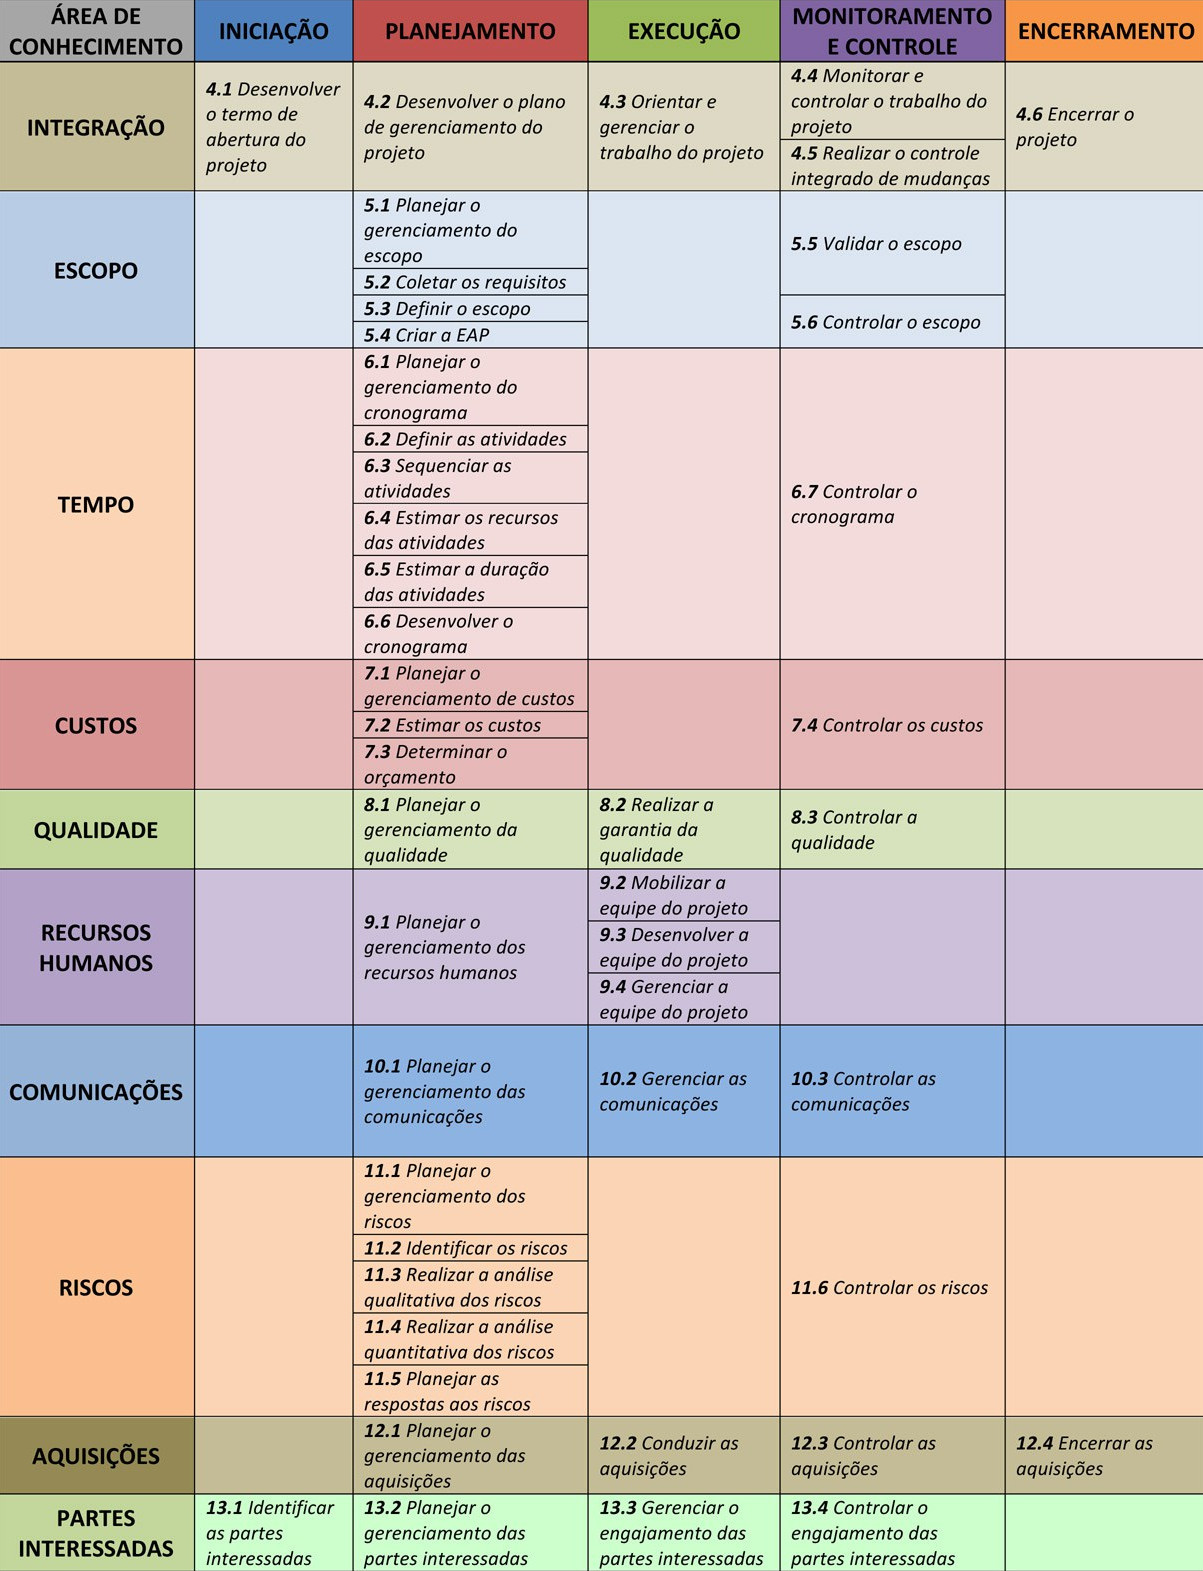
\includegraphics{figuras/processos_areas_pmbok}}
  \caption{Relação dos grupos de processos pelas àreas de conhecimento. Fonte: \cite{pmiguide2014}}
  \label{processos_areas_pmbok}
\end{figure}

Alguns autores afirmam que a garantia de que os objetivos definidos de projeto serão alcançados depende de um processo disciplinado, por parte da GP, que respeite custos, prazos e desempenho requeridos e que ocorra através do envolvimento de pessoas em atividades de planejamento e controle numa organização \cite{dinsmore2009ama, meredith2011project}.


\section{Sistemas de Gestão de Projeto}

Ao contrário do que é esperado pela natureza de negócios ou operações usuais, a natureza dos projetos e serviços é representada por processos curtos, repetitvos e funcionais, que facilitam a identificação de padrões usualmente inseridos em soluções de informação. Assim, especialista de GP veem o uso de sistemas de gestão de produtos (SGP), como uma ferramenta preciosa no que respeito a alcanço os objetivos e na excelência de projetos \cite{cserban2011project}.

Seguindo mais além, \citeonline{prado2006mmgp} afirma que diversos aspectos das metologias de GP dependem indiretamente do uso de SGP, sem que porém, seja determinada a natureza do SGP. O autor infere ainda que só é possível para organizações almejarem determinados níveis de maturidade se utilizarem essas ferramentas.

Através de um estudo quantitativo, \citeonline{liberatore2001project} analisou que nunca antes a adoção de uma ferramenta para auxiliar nas práticas de GP foi tão explorada quanto o uso de SGP. Os especialistas de GP demonstraram grande interesse pela facilidade encontrada no compreendimento da complexidade do projeto através desses sistemas, e expressaram interesse em integrar cada vez funcionalidades referente aos projetos.

Por meio de uma revisão na literatura \citeonline{hartmann2009implementing}, acrescentou que além de auxiliar no tratamento da complexidade nos projetos, o uso de SGP também se destaca para o aprimoramento da produtividade do processo de projeto, apesar de também ser notada uma dificuldade inicial para o adaptamento do uso dessas ferramentas.

Além de prover um meio para lidar com a produtividade de processo e complexidade do projeto, já foi comprovado também que o uso de SGP influi nos processos de planejamento, comunicação, monitoramento, controle de riscos, cronograma, gerenciamento de documentos e ainda avaliação de custos \cite{raymond2008project}.

Portanto, o uso de SGP implica em deter ferramentas capazes de facilitar e otimizar o esforço empregado pela GP para alcançar a excelência na realização do projeto, não apenas por parte do uso dos gestores do projeto, mas também por incluir outros atores presentes em seus processos \cite{cserban2011project}.


\section{Escritorio de Gestão de Projetos}

Advindo do inglês \textit{Project Management Office}(PMO), o escritório de gestão de projetos (EGP), ou ainda escritório de projetos (EP), pode ser considerado um conjunto de profissionais de GP que servem a um modelo organizacional com o propósito de aumentar a eficiência e lidar com as necessidades da GP, assumindo um papel de alta confiança ao implementar diversas estratégias em projetos \cite{kendall2003advanced}.

Através de um estudo, \citeonline{pemsel2013project} identificou três principais atividades que são esperadas do EGP:

\begin{itemize}
  \item Promover e facilitar o desenvolvimento estratégico da GP, bem como o uso estratégico de objetos que sejam empreendidos na GP;
  \item Planejar, controlar e dar suporte a GP, sempre assegurando que o conhecimento seja compartilhado no processo para melhorar sua eficiencia;
  \item Adoção estratégias de treinamento, negociação e formação para prover o desenvolvimento de competências.
\end{itemize}

Para \citeonline{dinsmore2005pmo} a principal expectativa empregada por um EGP esta relacionada ao suporte e orientação; ao processo de desenvolvimento e gerenciamento de projetos mais eficiente e eficaz o possível; e ao uso de metodologias e recursos de planejamento e análise de projetos padronizadas.

De acordo com \citeonline{crawford2010strategic}, por mais simples que um EGP possa ser, suas atividades compõem estruturas complexas responsáveis por atividades de planejamento, controle e monitoramento, cuja implantação representa um processo de mudança de cultura organizacional, por estar diretamente relacionada à negociação com pessoas. O autor retrata ainda três níveis de atuação do EGP que podem ser visualizados na figura \ref{pmo_crawford}.


\begin{figure}[ht]
  \centering
  \scalebox{0.6}{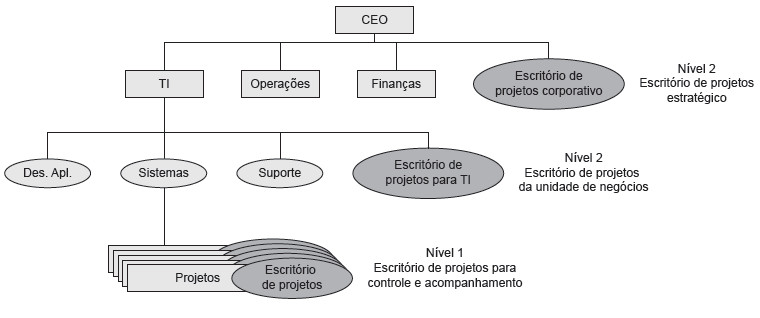
\includegraphics{figuras/pmo-crawford}}
  \caption{Níveis de atuação do escritório de projetos. Fonte: \cite{crawford2010strategic}.}
  \label{pmo_crawford}
\end{figure}

As competências desses níveis podem ser representas como \cite{crawford2010strategic}:

\begin{itemize}
  \item \textbf{Nível 1 - Escritório de Controle de Projetos:} visa o desenvolvimento do planejamente de projetos individualmente, realizando também a emissão de relatórios de progresso. Embora tenha foco em apenas um projeto, geralmente este projetos apresenta grande porte e complexidade;
  \item \textbf{Nível 2 - Escritório de Projetos da Unidade de Negócios:} oferece suporte a todos os projetos de uma área específica, porém de porte e complexidade variados;
  \item \textbf{Nível 3 - Escritório Estratégico de Projetos:} possui as seguintes competências:
  \begin{itemize}
    \item Selecionar, priorizar e garantir a integração de cada projeto para que esteja alinhado à estratégia da organização, inclusive no que respeito aos seus recursos;
    \item Desenvolver, atualizar e divulgar a metodologia de GP bem como seus conhecimentos;
    \item Converte-se em centro da gestão de conhecimento da organização através do armazenamento de informações sobre lições aprendidas;
    \item Validar estimativas de recursos realizadas pelo projetos, baseando-se em experiências anteriores.
  \end{itemize}
\end{itemize}

Assim, as responsabilidades de um EGP podem variar de acordo com a centralização empregada na organização, uma vez que está relacionada a padronização dos processos de GP. Entretanto as ferramentas e técnicas a serem empregadas ficam sob critério do gestor responsável pelo EGP \cite{pmiguide2014}.

Algums autores, ainda, apontam o EGP como uma ferramenta de apoio para que organizações obtenham bom desempenho em GP, bom como para alcançarem seus objetivos estratégicos. Esses mesmos autores destacam que fatores comuns ligados as taxas de sucesso do EGP, em caso positivo, devem ser enfatizados, enquanto em caso negativos, devem ser evitados, configurando assim boas práticas para o sucesso do EGP \cite{andersen2007benchmarking}.


\section{Gestão de Programas}

Programas podem ser entendidos por estruturas que consistem em uma equipe principal e um conjunto de equipes de projeto que averiguam capacidade de decisão e autoridade de um membro definitivo, isto é, um gerente de programa que assegura a direção e as decisões desta estrutura. Estas estruturas visam alcançar um determinado objetivo dentro de uma estratégia.\cite{brown2008handbook}.

\citeonline{rijke20141197} avalia que apesar da dificuldade geral em distinguir um programa de um projeto, a gestão de programas deve ser considerada mais extensa que gestão de projetos, pois ela abrange áreas em que projetos singulares não se encontram. Vale ressaltar também que o gestor de programa tem hábitos mais estrategicos que podem interferir na GP \cite{lycett2004289}.

Assim, a gestão de programas tem sido cada vez mais adotada por organizações com o objetivo de implementar estratégias que integrem melhor seus projetos e ferramentas, sem permitir que o desempenho possa desonrientar a natureza estratégica das decisões.


\section{Gestão de Portfólio}

A gestão de portfólio, conhecida também por Gestão de Portfólio de Projetos (GPP), surgiu a partir da necessidade de gerenciar investimentos em projetos nas organizações. Seu processo dinâmico e integrado visa avaliar o alinhamento estratégico e a viabilidade da execução simultânea de diversos projetos ao mesmo tempo. Esses projetos passam por uma introspecção que os seleciona e organiza de acordo com sua priorização em um portfólio \cite{meredith2011project, kerzner2013project}.

De acordo com \citeonline[p. 27]{burke2013project}, um portfólio pode abrigar conjuntos de projetos, programas e até mesmo outros portfólios que não precisam estar diretamente relacionados, mas que se reúnem por uma questão de otimização e controle. A figura \ref{port_prog_proj} demonstra sobre a relação entre portfólio, programas e projetos.

\begin{figure}[ht]
  \centering
  \scalebox{0.4}{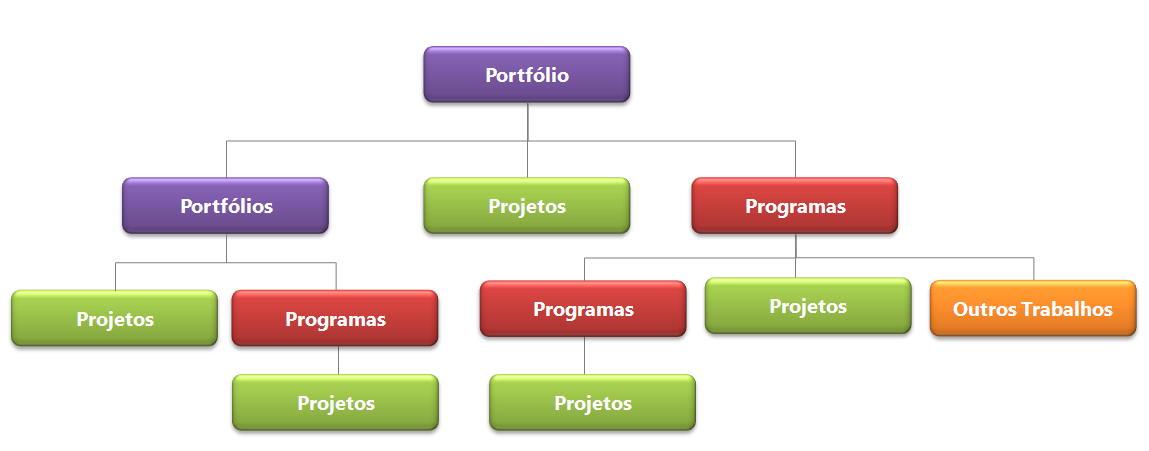
\includegraphics{figuras/port-prog-proj}}
  \caption{Relação Portfólio, Programas e Projetos. Fonte: \cite{pmi2006}}
  \label{port_prog_proj}
\end{figure}

\citeonline[p 11]{pmiguide2014} estabelece que o critério de agrupamento de um portfólio deve visar a facilitação na gestão para que seja possível atingir os objetivos estratégicos de uma organização. É definido ainda que toda gestão de portfólio fique sob responsabilidade de um EGP. A figura \ref{estrategia_portfolio} representa os processos incorporados pela Gestão de Portfólio.

\begin{figure}[ht]
  \centering
  \scalebox{0.4}{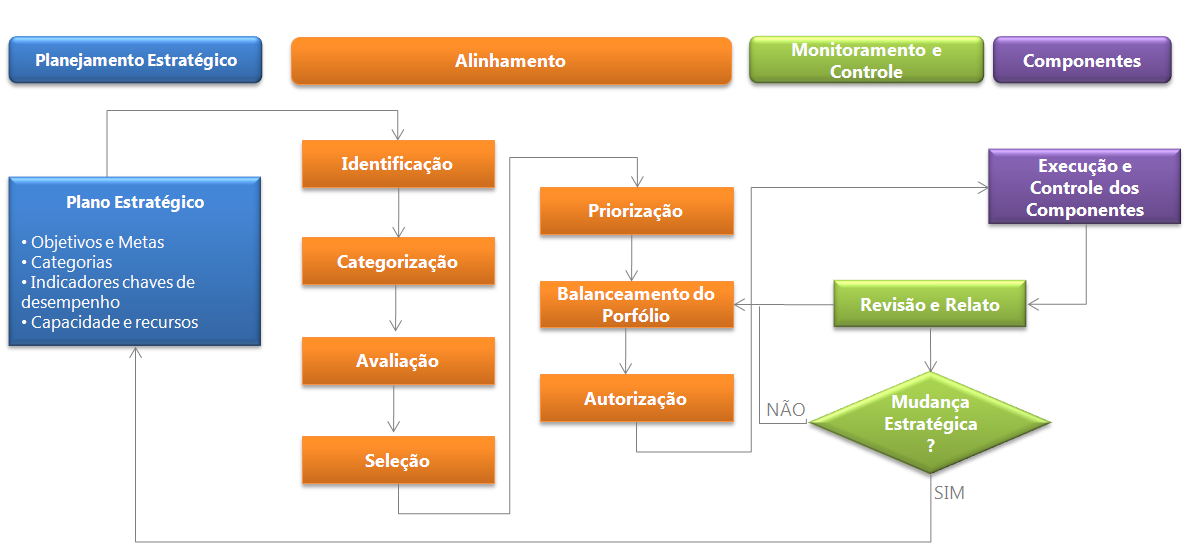
\includegraphics{figuras/estrategia-portfolio}}
  \caption{Processos de Gestão de Portfólio. Fonte: \cite{pmi2006}}
  \label{estrategia_portfolio}
\end{figure}

Desta forma, a GPP pode ser dita como uma manifestação de estratégia de negócios que determina os investimentos da organização via processos simultâneos, sistemáticos e dinâmicos de decisão, tornando o sucesso do EGP dependente do desempenho agregado de iniciativas dos componentes do portfólio e buscando a maximização do uso e do alinhamento desses componentes \cite{pmiguide2014}.

% \section{Gestão de Estratégica}
% \section{Maturidade em Gestão de Projetos}
% \section{Fatores Críticos de Sucesso}
 % Capitulo 2
% \chapter{A IMPORTÂNCIA DOS POLOS DE INOVAÇÃO}
\thispagestyle{empty}

\section{O modelo Universidade-Empresa-Governo}

Para \citeonline{saens2002ciencia} ciência pode ser definida por um método, uma instituição, uma tradição acumulativa de conhecimentos, um fator fundamental na manutenção e desenvolvimento da produção, e uma poderosa influência que deve refletir sua complexidade em diferentes aspectos na formação de crenças e atitudes relativas ao universo.

Compreende-se também que os avanços na ciência sempre estarão ligados a mudanças nas forças produtivas, e que por assim dizer estão diretamente ligados a inovação.

De acordo \citeonline{etzkowitz2003innovation}, a inovação pode ser linear, reversa, assistida ou interativa, ou um processo segue uma ordem natural em que a pesquisa científica básica, aplicada ou tecnológica será disponibilizado no mercado.

Em um modelo linear reverso as demandas da sociedade servem de ponto de iniciação de processo, enquanto no modelo linear assistido existe o desenvolvimento de mecanismos de apoio para a intermediação das capacidades de transferência de tecnologia, ou mesmo calculo de capital de risco. Existe ainda um modelo interativo que incorpora as características dos demais modelos, atendendo simultaneamente a diversas demandas e criando processos de apoio a inovação.

Nas últimas décadas os governos vêm criando incentivos a criação de ambientes de inovação, como incubadoras e projetos de pesquisa, que atuam dentro das universidades, sendo liderados muitas vezes pelos próprios projetos e com participação de empresas em diversos momentos, desde a criação desses projetos, ao oferecimento de mão de obra e/ou bolsas que suportem as pesquisas.

Essa missão que está voltada a trazer inovação para comunidade com bem competitivo e de eficiência veio através de um modelo desenvolvido a anos atrás.

Por volta do final dos anos 90, Henry Etzkovitz desenvolveu um modelo de inovação que visava explorar a relação UEG, este modelo veio a ser conhecido por tríplice hélice.

Neste modelo, as múltiplas relações consideradas recíprocas, eram dívidas em diferentes estágios de processo e disseminação de conhecimento de forma espiral, cada esfera representa uma instituição independente que trabalha em cooperação com as demais esferas, através de fluxos de conhecimento \cite{etzkowitz1998norms}.

\citeonline{etzkowitz2000dynamics} apresentaram uma visão da evolução dos SI, nas quais percebiam-se os conflitos potenciais nas relações de UEG. Portanto, essa nova visão trazia novas abordagens para essas variações nos arranjos institucionais dessas relações. A figura \ref{ueg_estatico} apresenta o modelo estático de relação UEG, onde o governo se envolve e passa a dirigir as relações entre as empresas e a Universidade.


\begin{figure}[ht]
  \centering
  \scalebox{0.7}{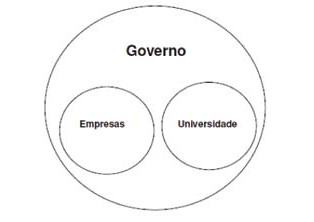
\includegraphics{figuras/ueg_estatico}}
  \caption{Modelo estático da relação UEG. Adaptado de \cite{etzkowitz2003innovation}.}
  \label{ueg_estatico}
\end{figure}

Uma segunda abordagem mostrada pela figura \ref{ueg_faire}, representa as relações completamente separadas entre as partes em suas esferas institucionais, assim estabelecendo relações por base de independência entre as partes. Essa abordagem também é conhecida por modelo “laissez-faire” de relação UEG.


\begin{figure}[ht]
  \centering
  \scalebox{0.7}{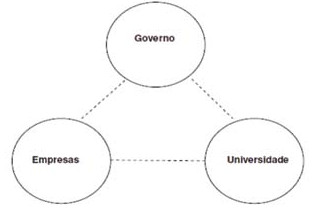
\includegraphics{figuras/ueg_faire}}
  \caption{Modelo \'laissez-faire\' da relação UEG. Adaptado de \cite{etzkowitz2003innovation}.}
  \label{ueg_faire}
\end{figure}

Na terceira abordagem, o conceito de geração de conhecimento é estruturado através da sobreposição das esferas institucionais, e portanto sobrepondo as ações das partes para estabelecer as condições de desenvolvimento de uma verdadeira relação produtiva. O objetivo é promover a inovação do ambiente na busca pelo conhecimento, pelo desenvolvimento econômico e por alianças estratégicas com empresas.

Neste memento o papel do governo deixa de ser controlar as outras esferas, e passa a ser estimular parcerias. Existe ainda um espaço para colaboração trilateral na formação de organizações híbridas, conforme visto na figura \ref{triplice_helice}.


\begin{figure}[ht]
  \centering
  \scalebox{0.7}{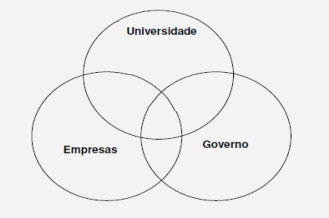
\includegraphics{figuras/triplice_helice}}
  \caption{Modelo da Tríplice Hélice na relação UEG. Adaptado de \cite{etzkowitz2003innovation}.}
  \label{triplice_helice}
\end{figure}

Neste último modelo também, universidade deixa de ser uma instituição centrada basicamente no ensino e combina seus recursos e potenciais na área de pesquisa com uma nova missão, desenvolver ideias de caráter econômico e social da sociedade, e assim estimula o surgimento de ambientes de inovação e dissemina uma cultura empreendedora.

Podem ser definidos como quatro os processos relacionados com as mudanças baseadas no conhecimento pela tríplice hélice \cite{etzkowitz2003innovation}:

\begin{itemize}
  \item{mudanças internas em cada esfera, tais como estratégias de cooperação ou alianças entre empresas concorrentes, ou a incorporação do desenvolvimento econômico e social como missão da universidade e o papel de articulador para o governo;}
  \item{reconhecimento da influência de cada esfera nas ações dos demais, seja essa influência por meio de legislações governamentais nas áreas de propriedade intelectual, ou transferência de tecnologia e inovação (Lei Bayh-Dole nos Estados Unidos e Lei da Inovação no Brasil);}
  \item{criação de novos relacionamentos entre as partes, sejam alianças estratégicas ou outras formas de cooperação que estimulem a criatividade e a inter-relação regional, e ainda a criação de ambientes de inovação;}
  \item{a ampliação e repercussão das ações da relação UEG junto à sociedade.}
\end{itemize}

Para \citeonline{etzkowitz1998norms} as universidades, e por assim dizer, formas de ensino, passaram por duas grandes revoluções desde a sua criação, época em que eram centradas na transmissão de conhecimentos dos professores para os alunos, sem um movimento de troca, apenas de repassamento de informações.

Na primeira revolução, que se deu no final do século 17, o conceito de pesquisa é agregado como missão das universidades, além das atividades de ensino. A princípio notou-se que muitos desafios ainda viriam antes de uma total incorporação das atividades de pesquisa no meio acadêmico.

Na segunda metade do século 20, mesmo com o ideal de pesquisa ainda não amadurecido, veio a segundo revolução que trouxe o conceito de Universidade empreendedora. Além da missão de ensino e pesquisa, neste memento mais um valor foi agregado como missão, o valor de formação de conhecimento voltado também ao desenvolvimento econômico e social.

Com este acréscimo a missão das universidades, houve uma proximidade entre essas e a sociedade, que começou a se sentir verdadeiramente inserida neste meio.

Alguns autores, como \citeonline{clark2003sustaining}, tratam a universidade empreendedora por Universidade inovadora, visto que a utilização de pesquisa e ciência permitem mudanças reais no mercado e portanto acarretam a inovação.

Assim, a concepção de universidade como simples “passadora” de conhecimento se modifica, se insere na sociedade, e passa a ser um dos principais papéis envolvidos na transformação de conhecimento gerado em valor econômico e social.

Entretanto, \citeonline{etzkowitz2003innovation} destaca que existem aspectos que prejudicam essa no época no ensino: na medida em que novos projetos surgem, conflitos de interesses também passar a surgir; esses conflitos de interesse podem ser decorrentes de interesses conflitantes, o não os ilegítima; assim a pesquisa e a comercialização dos resultados da pesquisa devem ser combinadas em um único modelo, visando evitar problemas.

Para \citeonline{clark2003sustaining} existem cinco fatores que endereçam questões críticas no processo de mudança nas universidades e portanto na relação UEG:

\begin{itemize}
  \item{a direção a seguir: no que respeito a estruturas gerenciais é preciso ter uma postura forte para que as mudanças sejam aceitas;}
  \item{o desenvolvimento expandido: é preciso estipular corretamente o desenvolvimento de novas estruturas frente as demandas da sociedade;}
  \item{as fontes de financiamento: diversificar as fontes de financiamento auxilia na ampliação dos recursos e portanto na estabilidade dos projetos;}
  \item{a estimulação das inovações: é preciso estimular os envolvidos nos processos de inovação para o processo seja bem aceito;}
  \item{a cultura empreendedora: é ideal criar uma cultura integrada, representada por uma visão compartilhada gerando uma perspectiva institucional.}
\end{itemize}

Assim, uma universidade empreendedora deve ser capaz de transformar pesquisa em resultados potenciais de comercialização, em ideias inovadoras tendo políticas de inovação como suporte de possibilidade de impacto regional.


\section{A relação UEG no Brasil}

No Brasil, durante os últimos 15 anos, tem existido um forte posicionamento em prol das atividades de PD\&I para inserção do meio acadêmico no dia a dia da sociedade frente as demandas da economia brasileira no mercado mundial e, desta forma, para estimular os SI, também entendidos como um conjunto de arranjos institucionais, cuja composição é dada pela relação UEG, levando à proposição de programas de incentivo à parceria \cite{vedovello2006capacidade, sbragia2006inovaccao}.

Entretanto, para \citeonline{toffler1990future}, nossos líderes políticos insistem no mito de o mercado, como sociedade industrial, esta destinado a perpetuar indefinidamente, e tristemente, muitos dos educadores, que por vezes são considerados agentes de mudança, dão continuidade a este pensamento. Assim, provavelmente, quando o futuro chegar junto a inovação essa ideia provará estar apenas obsoleta.

Essa preposição reforça que os SI sigam uma abordagem mais interativa, e menos linear, como o processo de empreendedorismo já antes citado por \citeonline{de2003introduccao}, que enfatiza um processo em que projetos podem ser apoiados por diferentes organizações, tanto privadas quanto governamentais.

Assim, podemos considerar que enquanto modelo de relação UEG, a tríplice hélice apresenta um arranjo organizacional bem evoluído por integrar a interação dessas três partes nos SI, e que serviu de ponto de partida para criação das Universidades Empreendedoras, como peças chaves para uma sociedade baseada no conhecimento \cite{etzkowitz2004evolution, etzkowitz2005innovating}.

No cenário internacional, diversos autores reconhecem o modelo da tríplice hélice como fator positivo no desenvolvimento regional e principal agente de inovação e transformação da ciência e tecnologia em crescimento econômico \cite{etzkowitz1998norms, etzkowitz2000dynamics, etzkowitz2007regional}.

Eles reconhecem ainda que esse crescimento da inovação esta diretamente ligado a capacidade de interação UEG prevista no modelo, bem como ao processo de aceitação da sociedade as mudanças na estrutura econômica.

Em suma, muitos estudos empíricos internacionais utilizaram seus esforços para estudar as relações e interações das partes frente a seu envolvimento, muitas vezes falhando em documentar sobre os aspectos da inovação em relação a sociedade.

\citeonline{tijssen2006universities} e \citeonline{welsh2008close} estudaram sobre como eram estabelecidas as relações entre as universidades e as empresas., \citeonline{campbell2005knowledge}, \citeonline{landry2006some}, \citeonline{mueller2006exploring} e \citeonline{welsh2008close} estudaram como se desenvolvia o recebimento e reinvestimento do suporte, ou fomento, recebido pelas universidades.

Por fim, sugeriram que a relação UEG pode afetar a performance e o desenvolvimento de ambas as partes de forma positiva, seja através da pesquisa, de patentes, ou desenvolvimento econômico \cite{landry2006some, mueller2006exploring, shane2004academic}.

\citeonline{sbragia2006inovaccao} avalia que no início, havia uma desconfiança mútua, fosse pela diferença de linguagem ou pelo choque de cultura, que resultava da falta de alinhamento entre as ideias e as imposições feitas pela pesquisa.

\citeonline{dagnino2003relaccao} levantaram um caso exemplar de relação UEG realizado pela Faculdade de Mecânica da Universidade Estadual de Campinas (FEM/Unicamp) com a então multinacional de autopeças Clark Equipaments. Inicialmente a proposta de interação veio através da realização de uma auditoria, posteriormente esta empresa se desenvolveu e se especializou de tal forma que veio a se desligar da filial se tornando Eaton Truck Corporation e vindo a firmar novos projetos tecnológicos com a participação da faculdade.

Através de um estudo que avaliou os dados do Diretório de pesquisa do CNPq no Censo 2002, \citeonline{rapini2007interaccao} destacou que existe a predominância de fluxos de conhecimento e serviços vindos de grupos de pesquisa para empresas, sendo esses serviços geralmente voltados a tarefas rotineiras de pouca complexidade. A autora destaca também que existe pouco uso do escopo de indicadores de CT\&I.

\citeonline{ipiranga2012tipo}, avaliaram a relação UEG através da Rede Nordeste Biotecnologia (Renorbio) e notaram que seu processo de cooperação era dotado de distinção de valores, linguagens, objetivos e cultura, o que tornava a interação entre as partes muito complexa, porém ativa para aqueles que estão diretamente envolvidos.

As autoras ainda destacam que um dos pontos que podem complexar a interação podem estar relacionados a falta de uma estrutura de gerenciamento, entretanto todos os resultados de pesquisa desenvolvidas estão patenteadas, demonstrando a viabilidade da inovação.

\citeonline{berni2015interaccao} relataram sobre a experiência vivida na Universidade Federal de Santa Maria (UFSM) pelo processo de incubadoras. De modo geral a experiência demonstrou ser positiva quanto a interação UEG, sendo mais voltado para as partes de universidade e empresa.

Para a empresa citou-se que houve auxílio ao desenvolvimento de novos produtos, enquanto para a universidade, houve o auxílio a formação de profissionais e possibilidades de direcionamento para aplicações práticas e interações com a comunidade.

\citeonline{etzkowitz2004evolution} e \citeonline{lundvall2010politicas} ressaltam que para alcançar o caminho da inovação é preciso cooperação de todas as partes, para que evoluam em um processo interativo e acumulativo que leva aos SI, sem cooperação não é possível compreender a distância entre o conhecimento e as diferentes  realidades da inovação.

Como \citeonline{ivanova2014rotational} ressaltam, é importante que o incentivo para o vinculo da relação UEG venha, sobretudo, da implementação de políticas governamentais, que tenham por objetivo garantir estrategias em diversas áreas que busquem a excelência e potencial contribuição para o crescimento econômico., assim como a melhoria de condição de vida no contexto regional e mesmo de nação \cite{lastres2005conhecimento}.

\section{A importância do PICG}

Para \citeonline{ristoff2011expansao} a Reforma Universitária garante que as universidades federais terão, enfim, a autonomia de gestão financeira prevista na constituição, mas nunca posta em prática; terão asseguradas a tão sonhada dotação global de recursos, a irredutibilidade nos repasses e a expansibilidade continuada.

Estarão, portanto, livres das amarras burocráticas e financeiras, que inibem a autogestão, repelem a inovação e forçam a privatização do espaço público. Ao defender a autonomia das universidades, nos termos do artigo 207 da Constituição, o governo também deixa claro o seu entendimento de que nestas instituições, embora não necessariamente nos Centros Universitários e Faculdades, as atividades de ensino, pesquisa e extensão são definidoras de sua natureza.

Em 2008, foram fundamentados os Institutos Federais (IF)\nomenclature{IF}{Institutos Federais} no país, para que fosse possível dar mais um passo no processo de expansão da Rede Federal de Educação, e também como parte dos objetivos de Plano de Desenvolvimento da Educação (PDE)\nomenclature{PDE}{Plano de Desenvolvimento da Educação} \cite{brasil2012ntextordmasculine, otranto2010criaccao}.

Um dos incentivos governamentais para conciliação de universidade, ou institutos, com empresas veio através da formalização da Empresa Brasileira de Pesquisa e Inovação Industrial (EMBRAPII)\nomenclature{EMBRAPII}{Empresa Brasileira de Pesquisa e Inovação Industrial} em 2013, para fomentar o processo de cooperação entre pequenas  e medias empresas nacionais e instituições tecnológicas ou privadas sem fins lucrativos.

Os primeiros projetos pilotos envolvem o Instituto de Pesquisa Tecnológico (IPT)\nomenclature{IPT}{Instituto de Pesquisa Tecnológico} na área de nanobiotecnologia, o Instituto Nacional de Tecnologia (INT)\nomenclature{INT}{Instituto Nacional de Tecnologia} em energia (gás/petróleo) e saúde e o Centro Integrado de Manufatura e Tecnologia (CIMATEC)\nomenclature{CIMATEC}{Centro Integrado de Manufatura e Tecnologia} do Serviço Nacional de Aprendizagem Industrial (SENAI)\nomenclature{SENAI}{Serviço Nacional de Aprendizagem Industrial} na área de automação manufatura.

Em março de 2015, a EMBRAPII selecionou cinco IF para atuarem em projetos de inovação industrial, para passarem pelo processo de seleção foi exigido das IF que participassem de um curso de capacitação de seus agentes de inovação, para que estivessem preparados para interagir com a relação UEG visando proporcionar eficiência  e agilidade no processo de transmissão de tecnologia para sociedade \cite{embrapiiff}.

Entre os polos selecionados destacasse o Polo de Inovação Campos dos Goytacazes pertencente ao Instituto Federal Fluminense (IFF)\nomenclature{IFF}{Instituto Federal Fluminense} em parceria com o Campus Rio Paraíba do Sul (UPEA)\nomenclature{UPEA}{Campus Rio Paraíba do Sul}, inicialmente Unidade de Pesquisa e Extensão Agroambiental.

Atualmente conhecido por PICG, o polo está localizado no município de Campos dos Goytacazes – RJ, no norte do estado do Rio de Janeiro, e foi reconhecido pelo Ministério da Educação em 13 de agosto de 2015 (PICG/IFFluminense – Portaria 819/2015). Desde sua inauguração a UPEA vem  realizando diversos trabalhos de fundamento ambiental para o atendimento das demandas regionais \cite{embrapiiff}.

Neste memento o PICG está sendo estruturado para desenvolver projeto de PD\&I e receberá um financiamento de R\$ 3 milhões para um plano de ação de 3 anos. Este plano de ação contará diretamente com a participação de empresas da região, visando transferir tecnologia para essas e, por fim, para a sociedade local \cite{embrapiiff}.
 % Capitulo 3
\chapter{ESTUDO DE CASO}
\thispagestyle{empty}

\section{A natureza de pesquisa}

Esta pesquisa pode ser caracterizada como uma pesquisa bibliográfica, cujo método utilizado foi o estudo de caso. Visando atingir o objetivo da pesquisa, inicialmente, foi realizada uma pesquisa bibliográfica através do material existente na literatura.

Através da leitura foi possivel identificar os elementos de pesquisa propostos por \citeonline{lakatos2010fundamentos}, são eles: intenção, reflexão espírito crítico, atenção, análise e síntese.

Se utilizada a proposta de \citeonline{gil2002elaborar}, a presente pesquisa é tomada por qualitativa quanto a abordagem da problemática, e descritiva quanto a caracterização de seus objetivos, pois utiliza do desenvolvimento de um estudo de caso.

\citeonline[p 239]{fortin2009fundamentos} confirma que todo estudo que objetiva a identificação de características referentes a um fenómeno, visando obter uma visão geral de sua situação ou população em questão, pode ser apresentado como um estudo descritivo. Nestas condições, determinado trabalho consistirá na pretenção de descrever ou interpretar a propriedades desta investigação, através de análises empíricas e da descrição da problemática \cite{fortin2009fundamentos, lakatos2010fundamentos}.

\section{Método de Pesquisa}

Para \citeonline{de2007metodologia} todo e qualquer trabalho científico deve proporcionar a reprodução de experiências de modo que outros pesquisadores sejam capazes de obter resultados descritivos, de repetir suas observações e ainda de realizar julgamentos as conclusões de seu(s) autor(es).

De acordo com \citeonline{vergara2009projetos} pesquisas também podem ser caracterizadas em relação aos aspectos relativos aos fins e aos meios. A presente pesquisa influe no carater exploratório descritivo quanto aos fins, pois se enquadra expõem características de uma determinada população, sem o compromisso de explicar os fenômenos que descreve, embora sirva de base para essa explicação.

Assim, porque é de pretensão deste trabalho descrever e interpretar, mas do que avaliar um caso real presente, e seguindo o caráter de investigação revelado por \citeonline{fortin2009fundamentos}, este trabalhor se apresenta como descritivo e exploratório.

Por sua vez, quanto aos procedimentos técnicos que foram utilizados para obtenção dos dados, seguindo a classificação proposta por \citeonline{lakatos2010fundamentos}, trata-se de pesquisa bibliográfica, que também pretende utilizar de uma pesquisa de campo.Uma pesquisa de campo é aquela que busca alcançar informações referentes a um problema e busca uma resposta ou de uma hipótese, que se pretende comprovar, bem como descobrir novos fenômenos ou as relações entre eles \cite{de2007metodologia}.


\section{População e Amonstragem}

\citeonline[p 20]{de2011elaboraccao} define população pesquisa como aqueles a que ela se refera ou representa, isto é, o universo compreendido dentro da pesquisa. Nesta pesquisa, o universo abordado se refere aos funcionários envolvidos no processo de construção do escritório de projetos do PICG.

Para atender a discussão científica proposta no presente estudo, de acordo com a posição de \citeonline{vergara2009projetos}, foi apresentada uma problemática referente ao universo que será exposta no próximo capítulo.
 % Capitulo 4
\chapter{CONSIDERAÇÕES FINAIS}
\thispagestyle{empty}

Ao consultar o Portal de Inovação e Diretório de dados do CNPq, é possível notar que o Brasil possui inúmeros pesquisadores em diversas áreas do conhecimento, bem como diversos projetos de pesquisa, incubadoras e parques tecnológicos dignos de primeiro mundo.

Este trabalho apresentou uma perspectiva sobre um novo modelo de parceria entre a EMBRAPII e o PICG envolvendo critérios respectivos a gestão de projetos em um escritórioa de projetos voltado a ações de PD\&I.

Para atender as expectativas de inovação e competitividade impostas ao PICG, este trabalho irá buscar verificar o uso de conceito e ferramentas de gestão de projetos empregados no escritório de projetos, através de um mapeamento com base no modelo de maturidade imposto pela EMBRAPII.


\newpage
\thispagestyle{empty}
\singlespacing
\section{Cronograma}

\begin{enumerate}
  \item{Contato – Equipe Administrativa do Polo de Inovação Campos dos Goytacazes (PICG);}
  \item{Participação treinamento de GP do PICG;}
  \item{Revisão Bibliográfica;}
  \item{Coleta de dados – escritório de projetos;}
  \item{Roteirização;}
  \item{Defesa do Projeto;}
  \item{Análise dos Indicadores dos projetos do PMO;}
  \item{Discussão sobre análise;}
  \item{Mapeamento do Modelo de Maturidade EMBRAPII;}
  \item{Discussão dos Resultados;}
  \item{Revisão do projeto final;}
  \item{Defesa.}
\end{enumerate}

\begin{table}[!htpb]
  \centering
  \begin{small}
    \setlength{\tabcolsep}{4pt}
    \begin{tabular}{|c|c|c|c|c|c|c|c|c|c|c|c|c|c|c|c|c|c|c|c|}\hline
      & \multicolumn{19}{c|}{Meses (2015 - 2016 - 2017)}\\ \cline{2-20}
      \raisebox{1.5ex}{Etapa} & ago & set & out & nov & dez & jan & fev & mar & abr & mai & jun & jul & ago & set & out & nov & dez & jan & fev \\ \hline
      1 & X &   &   &   &   &   &   &   &   &   &   &   &   &   &   &   &   &  &  \\ \hline
      2 & X & X & X & X & X & X &   &   &   &   &   &   &   &   &   &   &   &  &  \\ \hline
      3 &   &   & X & X & X & X & X & X & X & X & X & X &   &   &   &   &   &  &  \\ \hline
      4 &   &   &   &   &   &   &   &   & X & X &   &   &   &   &   &   &   &  &  \\ \hline
      5 &   &   &   &   &   &   &   &   &   & X & X &   &   &   &   &   &   &  &  \\ \hline
      6 &   &   &   &   &   &   &   &   &   &   &   &   & X &   &   &   &   &  &  \\ \hline
      7 &   &   &   &   &   &   &   &   &   &   &   & X & X & X &   &   &   &  &  \\ \hline
      8 &   &   &   &   &   &   &   &   &   &   &   &   &   & X & X &   &   &  &  \\ \hline
      9 &   &   &   &   &   &   &   &   &   &   &   &   &   &   & X & X &   &  &  \\ \hline
      10 &  &   &   &   &   &   &   &   &   &   &   &   &   &   &   & X & X &  &  \\ \hline
      11 &  &   &   &   &   &   &   &   &   &   &   &   &   &   &   &   & X & X &  \\ \hline
      12 &  &   &   &   &   &   &   &   &   &   &   &   &   &   &   &   &   &  & X \\ \hline
    \end{tabular}
  \end{small}
  \caption{Cronograma das atividades previstas}
  \label{t_cronograma}
\end{table}

 % Capitulo 5

\bibliography{referencia} % Gera as referências bibliográficas
\apendice
\chapter{ANÁLISE BIBLIOMÉTRICA}

A bibliometria foi realizada por meio do levantamento bibliográfico relacionado ao tema da pesquisa, utilizando o mecanismo de busca Google Acadêmico, e as bases de periódicos da CAPES, \textit{SCOPUS} e \textit{ScienceDirect}. As principais expressões de busca utilizadas foram: ``project management'' , ``project management agile'', ``agile'' e a tradução destas para a língua portuguesa. A seguir será apresentado os passos desta análise.

\section{Material não disponibilizado pela base CAPES}

O levantamento bibliográfico das fontes impressas e digitais, que não se encontravam disponiveis pela Portal Capes, foi realizado através do portal \textit{ScienceDirect} e do mecanismo Google Acadêmico, que dispõe de bancos de teses e dissertações de instituições específicas, e aprensenta redirecionamento às bases Biblioteca Digital Brasileira de Teses e Dissertações (BDTD), Scientific Electronic Library Online (SciELO).

Ressalta-se ainda que o mecanismo de busca Google Acadêmico também indexa em suas pesquisas as bases de periódicos da CAPES, \textit{SCOPUS} e \textit{ScienceDirect}, permitindo ao usuário avaliar a relevância de citações de um determinado periódico em ambas as bases, e redirecionando o usuário as bases para leitura dos períodicos.

Foi realizada também, uma pesquisa sobre o tema para saber sobre o interesse no mesmo nos ultímos anos, para tanto foi utilizada a ferramenta Google \textit{Trends}. Primeiramente foi utilizada a frase de pesquisa ``project management'' para demonstrar o interesse específico sobre as práticas de GP. O resultado apresentado no gráfico \ref{trends1}, que parte do ano de 2006, declinando em pesquisas até o ano de 2016.


\begin{figure}[!ht]
  \centering
  \scalebox{0.5}{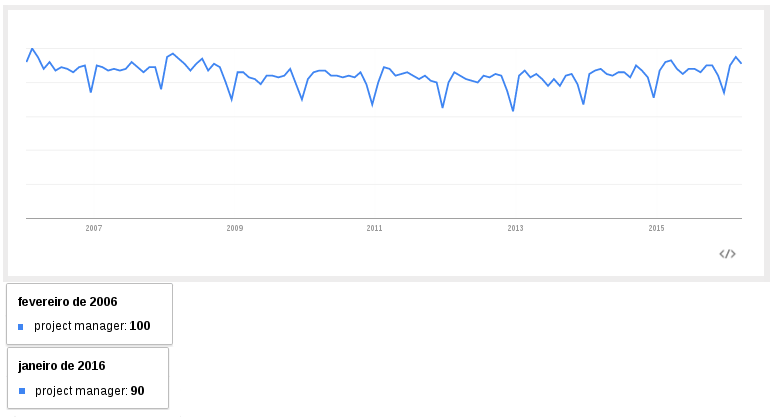
\includegraphics{figuras/trends1}}
  \caption{Interesse sobre práticas de GP ao passar do tempo. Fonte: Google \textit{Trends} (2016).}
  \label{trends1}
\end{figure}


Para saber o interesse sobre práticas de GP que fossem consideradas agéis foi somada a pesquisa a frase ``project management agile'', para que assim pudesse haver um comparação sobre o interesse dessas práticas com o passar do tempo. O resultado desta pesquisa é apontado no gráfico \ref{trends2}, onde o interesse pela gestão de projetos apresenta um declinío lento, enquanto o interesse pela gestão ágil de projetos cresce, também lentamente.

\begin{figure}[!ht]
  \centering
  \scalebox{0.5}{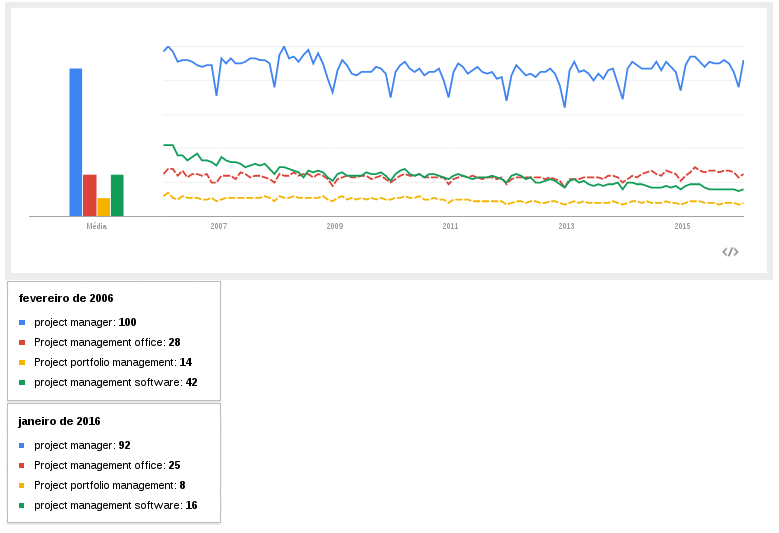
\includegraphics{figuras/trends2}}
  \caption{Interesse sobre práticas de GP versus práticas agéis ao passar do tempo. Fonte: Google \textit{Trends} (2016).}
  \label{trends2}
\end{figure}


Os indicadores bibliométricos escolhidos foram os seguintes: ano de publicação, idiomas, autores e tipos de documento. Seguindo os indicadores escolhidos, a seleção dos artigos foi feita considerando os seguintes critérios:

\begin{itemize}
  \item \textbf{Ano de Publicação:} foi considerado o periodo de 2005 a 2015, isto é, a equivalências aos ultimos dez anos, pois entende-se que este periodo compreende os anos de maior interesse no tema de pesquisa de acordo com mecanismo utilizado.
  \item \textbf{Idiomas:} foi dada preferência ao inglês pela importancia que os períodicos desse idioma representaram, entretanto também foram escolhidos períodicos em português pela sua relevância ao tema proposto.
  \item \textbf{Autores:} foram consideradas principalmente publicações de autores mais pesquisados e mais citados.
  \item \textbf{Tipos de Documento:} foi dada preferência a publicações em periodicos, por traduzirem pensamentos mais recentes relativos ao tema de pesquisa.
\end{itemize}


Os trabalhos selecionados a partir da análise bibliometrica, após a aplicação dos indicadores mencionados, encontram-se relacionados no quadro \ref{tabela_autores}.

\begin{longtable}{| p{.20\textwidth} | p{.80\textwidth} |}
  \cline{1-2}
  \cellcolor[HTML]{C0C0C0}{\color[HTML]{000000} Autor(es)} & \cellcolor[HTML]{C0C0C0}{\color[HTML]{000000} Publicação} \\ \hline
  ALMEIDA, L. F. M. et al. & Fatores críticos da agilidade no gerenciamento de projetos de desenvolvimento de novos produtos (2012) \\ \hline
  AMARAL, D. C. et al. & Gerenciamento ágil de projetos: aplicação em produtos inovadores (2011). \\ \hline
  ATKINSON, R. D.; EZELL, S. J.; STEWART, L. A. & The global innovation policy index(2012). \\ \hline
  BARLOW, J. B. et al. & Overview and guidance on agile development in large organizations(2011). \\ \hline
  BATRA, D. et al. & Balancing agile and structured development approaches to successfully manage large distributed software projects: A case study from the cruise line industry(2010). \\ \hline
  BECK, K. et al. & Manifesto for agile software development(2001). \\ \hline
  BERGGREN, C.; SÖDERLUND, J. & Rethinking project management education: Social twists and knowledge co-production(2008). \\ \hline
  BINDER, J.; AILLAUD, L. I.; SCHILLI, L. & The project management cocktail model: An approach for balancing agile and iso 21500(2014). \\ \hline
  BOEHM, B.; TURNER, R. & Management challenges to implementing agile processes in traditional development organizations(2005). \\ \hline
  CAMPBELL, D. F.; GUTTEL, W. H. & Knowledge production of firms: research networks and the"scientification"of business r\&d(2005). \\ \hline
  CICMIL, S. J. et al. & Exploring the complexity of projects: Implications of complexity theory for project management practice(2009). \\ \hline
  COCKBURN, A. & Agile software development(2006). \\ \hline
  COLLYER, S. et al. & Aim, fire, aim—project planning styles in dynamic environments(2010). \\ \hline
  CONFORTO, E. C.; AMARAL, D. C. & Evaluating an agile method for planning and controlling innovative projects(2010). \\ \hline
  ETZKOWITZ, H.; KLOFSTEN, M. & The innovating region: toward a theory of knowledge-based regional development(2005). \\ \hline
  FERNANDEZ, D. J.; FERNANDEZ, J. D. & Agile project management—agilism versus traditional approaches(2008). \\ \hline
  GANGULY, A.; NILCHIANI, R.; FARR, J. V. & Evaluating agility in corporate enterprises(2009). \\ \hline
  GERALDI, J. G. et al. & Innovation in project management: Voices of researchers(2008). \\ \hline
  HASS, K. B. & The blending of traditional and agile project management(2007). \\ \hline
  HIGHSMITH, J.; COCKBURN, A. & Agile software development: The business of innovation(2009). \\ \hline
  KOLLTVEIT, B. J.; KARLSEN, J. T.; GRØNHAUG, K. & Perspectives on project management(2007). \\ \hline
  LASTRES, H. M.; CASSIOLATO, J. E.; ARROIO, A. & Conhecimento, sistemas de inovação e desenvolvimento(2005). \\ \hline
  LEYBOURNE, S. A. & Improvisation and agile project management: a comparative consideration(2009). \\ \hline
  MIR, F. A.; PINNINGTON, A. H. & Exploring the value of project management: linking project management performance and project success(2014). \\ \hline
  QUMER, A.; HENDERSON-SELLERS, B. & An evaluation of the degree of agility in six agile methods and its applicability for method engineering(2010). \\ \hline
  STARE, A. & Agile project management in product development projects(2014). \\ \hline
  STYHRE, A. & The bureaucratization of the project manager function: The case of the construction industry(2006). \\ \hline
  WILLIAMS, T. & Assessing and moving on from the dominant project management discourse in the light of project overruns(2005). \\ \hline
  WINTER, M. et al. & Directions for future research in project management: The main findings of a uk government-funded research network(2006). \\ \hline
  \caption{Publicações Selecionadas. Autoria própria (2016).}
  \label{tabela_autores}
\end{longtable}
 % Inclui Apendices
\anexo
\chapter{ARTIGO}

\begin{center}
{\large \textbf{Do tradicional ao ágil: uma perspectiva do gerenciamento de projetos}}
\end{center}

\begin{center}
\textbf{RESUMO}
\end{center}

\singlespacing
\noindent A chegada da era da inovação no mercado impôs diversas mudanças ao mundo, entre elas às práticas de gerenciamento de projetos, ou a sua versão tradicional, como ficou conhecida. Para lidar com a necessidade constante de modificações ao longo de projetos novas abordagens foram pautadas, de Gerenciamento Ágil de Projetos (GAP). Entretanto, a existência de estudos que comprovem a total eficácia do uso dessas abordagens ainda é escassa. Este artigo apresenta uma revisão bibliográfica de estudos que visaram divulgar essas abordagens, apontando vantagens e desvantagens de seu uso, e ainda de trabalhos que utilizaram técnicas de ambas abordagens, propondo novos modelos de seu uso. É possível argumentar que muitos projetos ainda não utilizam nenhuma abordagem, e que para os que utilizam abordagens tradicionais, a mesclagem com abordagens GAP são aconselháveis. \\
\noindent Palavras-chave:


\begin{center}
\textbf{ABSTRACT}
\end{center}

\singlespacing
\noindent The arrival of the era of innovation in the market requires several changes to the world, including the project management practices, or the traditional version, as it became known. To cope with the constant need to change along new approaches projects were guided in Agile Project Management (APM). However, there are studies that prove the overall effectiveness of the use of these approaches is still scarce. This article presents a literature review of studies that aimed to disseminate these approaches, indicating advantages and disadvantages of their use, and still works using techniques of both approaches, proposing new models of its use. It is possible to argue that many projects still do not use any approach, and to those using tradicional approaches, merging with APM approaches are advisable. \\
\noindent Keywords:


\onehalfspacing

\section{INTRODUÇÃO}

Com a chegada do século 21, o mundo enfrentou diversas mudanças, tanto com respeito as inovações tecnológicas quanto ao cenário no mercado produtivo. Custo e qualidade deixaram de ser a principal motivação de melhoria nas empresas, cedendo espaço para projetos que entreguem produtos mais flexíveis em menor espaço de tempo (Yusuf 2004).

Neste contexto foi possível destacar a importância da inovação, do atendimento as constantes modificações de requisitos por parte dos clientes e ainda importância de manter o cliente como alvo da organização, para conquistá-lo e gerar vínculos de fidelização (CHIESA, 2007).

Na busca por soluções que tornassem possível a sobrevivência neste ambiente desafiador e imprevisível, a indústria decidiu voltar-se ao gerenciamento de projetos (GP), que no entanto, de acordo com Geraldi (2008), mostrou-se incapaz de lidar com tais mudanças a princípio.

Para Lin (2006) as ferramentas e técnicas tradicionais empregadas no GP não previam atividades de inovação nem instabilidades durante o processo de seus produtos, pois previam projetos linear e sem inconstâncias.

Visando atender a expectativa de mercado e a melhoraria da gestão de projetos, abordagens alternativas, que vinham se desenvolvendo desde o início dos anos 90, com novos princípios, ferramentas e técnicas, pareceram a melhor resposta. Essas abordagens vieram a ser conhecidas por Gerenciamento Ágil de Projetos (GAP) (Amaral 2011).

Entretanto é preciso que haja melhor compreensão sobre cada abordagem no que respeito aos processos executados na formação dos produtos em seu meio, e verificada adaptação destas abordagens.

Este artigo visa apresentar uma revisão bibliográfica sobre a transição das abordagens de GP, nas primeiras seções se apresentam as definições básicas de cada abordagem, seguido por uma seção de análise de estudos realizados na utilização dessas abordagens, e por fim as conclusões referentes a esta pesquisa.

\section{GERECIAMENTO DE PROJETOS}

Por definição, um projeto pode ser considerado um conjunto de atividades temporárias empregadas sobre recursos com a finalidade de entregar um serviço ou produto único (STELLINGWERF 2013). De acordo com o Instituto de Gerenciamento de Projetos (PMI, 2014), uma metodologia de GP deve conter um conjunto de métodos, técnicas, procedimentos, regras, modelos e boas práticas que possam ser usadas em projetos.

O uso dessas metodologias se tornou comum por volta do ano de 1950, e desde então vem se popularizando e tomando forma a medida que o mercado demonstra a necessidade de seu uso (Garel, 2013).

Para Eder (2012) a composição de uma ação, ou ato que gere resultados através do uso de um conjunto de técnicas e ferramentas, ou ainda um conjunto de artefatos que possam ser utilizados como ferramentas, descreve uma prática.

Dinsmore (2009) o GP deve ser realizado através de processos como iniciar, planeja, executar, controlar e encerrar, e deve contar com o uso de recursos como conhecimentos, habilidades, ferramentas e técnicas em atividades de projetos a fim de satisfazer seus requisitos.

Do ponto de vista de Charvat (2003), uma metodologia de GP representa um composto de orientações e princípios que podem ser adaptados e aplicados a situações específicas, onde este composto pode ser representado por uma simples lista de tarefas ou um conjunto de ferramentas e técnicas.

Para Shenhar (2007), o GP visa atingir tarefas e metas previstas em um plano estratégico de uma organização e serve de abordagem para a interação entre projetos, estratégia e objetivos organizacionais.

Similarmente, Cockburn (2000) define processo de software como um conjunto de ferramentas e práticas usadas para o desenvolvimento de produtos, e define GP como o conjunto de princípios que visa entregar um produto com sucesso.

Garel (2013) vê as metodologias de GP como conhecimento expresso em tarefas, técnicas, funções, ferramentas e entregas ao longo de um projeto em curso, que se utiliza de conhecimento sobre ajustes.

Em suma, todas metodologias de GP são similares enquanto se baseiam em abordagens, princípios e regras para satisfazer requisitos e entregar produtos de qualidade com sucesso.


\subsection{GERECIAMENTO DE PROJETOS TRADICIONAL}

Ao decorrer dos anos, as abordagens de GP foram disseminadas como “guias de conhecimento”, que apresentavam um conjunto de técnicas, princípios, ações e ferramentas que supostamente seriam capazes de gerenciar qualquer projeto (Kolltveit, 2007; Shenhar, 2007).

Inicialmente essas abordagens mantinham o foco no planejamento e controle do produto de forma engessada sem prever instabilidade e emergências, pois acreditava que era importante entregar o produto de acordo com os requisitos previamente levantados, indiferente a dissociações naturais do dia a dia (Winter, 2006).

Shenhar (2007) afirma que alguns autores investigaram sobre a correlação das práticas adotadas de acordo com o tipo de projeto descrito e das ferramentas utilizadas, e constataram que grande parte dos projetos eram geridos sem a devida diferenciação quanto a sua natureza, e com o uso de práticas genéricas denominadas “melhores práticas”.

De acordo com Collyer (2010) foi reconhecido pelo PMBOK que as práticas deveriam prever planos emergências que lidassem com conformidades não previstas nos requisitos, entretanto quanto a formação da ISO 21500, utilizada como padrão pela GP, nota-se que suas técnicas e ferramentas referiam-se com frequência ao modelo Cascata, quanto ao ciclo de vida do projeto apresentado por Boehm (1988).

Como explica Almeida (2012), é natural que práticas e abordagens evoluam ao longo dos tempos, como projetos passaram a ser o centro de toda e qualquer organização, entretanto, notou-se que a prática de GP se mantinha inadequada e que grande parte das falhas gerências estavam diretamente ligadas as técnicas utilizadas nestas praticas de GP.

A motivação das abordagens de GP consideradas tradicionais estava diretamente relacionada a perspectiva de que projetos eram relativamente simples, previsíveis eque seguiam de forma linear, tornando-os fáceis de detalhar e seguir ao longo do planejamento. Possibilitando assim, uma entrega eficiente dentro do prazo. (Andersen, 2006; Boehm, 2002; Boehm \& Turner, 2003; Cicmil, 2009; Collyer, 2010; Leffingwell, 2007; Shenhar, 2007; Williams, 2005; Wysocki, 2011).

Ainda, uma das vantagens descritas na prática tradicional era a capacidade robusta, isto é, a defesa de que diversos projetos poderiam sempre ser gerenciados seguindo as mesmas técnicas e ferramentas, como se fossem todos na mesma natureza.

Para diversos autores (Aguanno, 2004; Cicmil, 2009; Chin 2004; Shenhar, 2007; Williams, 2005; Wysocki, 2011) a robustez de planejamento é a maior desvantagem da prática tradicional, pois projetos têm se tornado cada vez mais complexo, e o para ideal de planejar linearmente não compete lidar com irregularidades dinâmicas da realizada do mercado.

Entretanto, Styhre (2006) destaca que no desejo por diminuir riscos e evitar ineficiências, o foco de gerenciar criatividade e mudanças é burocratizado e acaba por ser tornar um gerenciamento de papéis e formulários, geralmente encontrados na robustez do projeto.

Outra desvantagem notada é que por focar no planejamento e controle, essas abordagens ignoram não só a natureza do projeto, como também aspectos humanos quanto a sociabilização, contextualização e tendência a mudanças (Winter, 2006; Highsmith, 2009).

\subsection{GERENCIAMENTO DE PROJETOS ÁGIL}

Em função as desvantagens apontadas nas abordagens tradicionais de GP, somadas ao crescimento de um mercado inovador, com demandas contínuas e necessidade pela redução de custos, resultaram no advento de novas abordagens para GP (Aguanno, 2004; Conforto \& Amaral, 2010; Williams, 2005).

Em 2001, a partir de uma iniciativa em conjunto conhecida por Manifesto Ágil houve a formalização das abordagens ágeis. Seu diferencial se apresentava, simplificadamente, como um conjunto de técnicas, princípios e ferramentas que melhoravam o trabalho em time, permitindo adaptação e evoluções ao longo do projeto (Beck et al., 2001; Berggren, 2008; Cohn, 2005; Hass, 2007; Highsmith, 2009; Fernandez, 2008; Fitsilis, 2008; Larman, 2003; Salomo, 2007; Schwaber, 2004; Smith, 2007; Qumer, 2010).

De acordo com Cockburn (2000) e Schwaber (2001) existem quatro princípios ágeis que devem sempre ser enfatizados:
1. Indivíduos e Interações são mais importantes que processos e ferramentas;
2. Colaboração com as necessidades dos clientes acima de negociação de contratos;
3. Produto em funcionamento vale mais que documentação abrangente;
4. Responder as mudanças independente do plano a seguir.

Existem também práticas e ferramentas, como a concepção de visão do produto, desenvolvimento iterativo; além do uso de ferramentas visuais de planejamento do projeto e de seus artefatos (Augustine, 2005; Boehm \& Turner, 2004; Chin, 2004; Highsmith, 2009).

Ao ressaltar a importância dos itens, entretanto, os autores destacam que eles não se excluem, o ideal é que todos sejam levados em consideração, apenas seguindo a ordem de importância (Aguanno, 2004).

Essas abordagens podem ser apontadas por GAP, e representaram uma alternativa para problemática das mudanças constantes, alterações a curto prazo dentro do planejamento do projeto, valorização do cliente como uma fonte de interação (Amaral, 2011; Augustine, 2005; Cohn, 2005; Highsmith, 2009).

Alguns autores (Aguanno, 2004; Boehm, 1988; Manifesto, 2001; Williams, 2005), enfatizam que estas abordagens têm uma relação muito estreita com a engenharia de software, levando essas abordagens a aparecerem com frequência relacionadas ao desenvolvimento de software.

Stare (2014) afirma que durante uma entrevista os autores responsáveis pelo Manifesto Ágil ressaltaram a importância das abordagens GAP como um meio de tornar o GP uma ferramenta de sucesso no atual mercado, e que apesar de serem inicialmente aplicadas em projetos de tecnologia de informação (TI), eram igualmente apropriadas a qualquer natureza de projetos, visto que o foco destas abordagens está em reconhecer e aplicar feedback com a finalidade de lidar com incertezas.

Apesar desta declaração, Stare (2014) contesta que nos estudos pesquisados até o ano de 2009, em sua maioria, as práticas ágeis se referiam ao uso em projetos de TI, e que neste ano, algumas pesquisas começaram a reconhecê-las em outros campos com certo receio.

Entre as metodologias ágeis mais utilizadas, as que mais se destacam na indústria são: Scrum (Schwaber, 2004), Lean Software Development (Poppendieck, 2003), Crystal (Cockburn, 2004), Feature Driven Development (Palmer, 2002), Adaptive Software Development (Highsmith, 2001) e eXtreme Programming (Beck, 2000).

Considerando a crescente necessidade da indústria por inovação e pela necessidade de redução de custos, as abordagens GAP tomaram o cenário de GP devido sua habilidade de adaptação durante o ciclo de vida dos projetos, indiferente a sua natureza. Mudanças são inevitáveis e impossíveis de prever, portanto é importante lidar com elas (Aguanno, 2004; Conforto \& Amaral, 2010; Chin, 2004; DeCarlo, 2004; Highsmith, 2009; Leffingwell, 2007; Williams, 2005).

Além disso, como atrativos para utilização de práticas ágeis se destacam: a melhora na habilidade de comunicação formal e informal, bem como a colaboração externa com a aproximação dos clientes no processo de produtos (Aguanno, 2004; Cockburn, 2006; Collyer., 2010; Coram, 2005; DeCarlo, 2004; Highsmith, 2001; Williams, 2005).

Alguns autores destacam que a proximidade do time com o projeto melhora seu desempenho e a habilidade de ser autogerenciáveis e responsáveis em suas tarefas (Augustine, 2005; Boehm \& Turner, 2004; Highsmith, 2009).

Vale destacar que também existiram ideias de foram herdadas das práticas tradicionais, como o ideal de que o projeto fosse iterativo, isto é, pudesse ser incrementado ao longo do processo de produção (Boehm, 1988; Aguanno, 2004).

Entretanto, invés de utilizar um único plano para o projeto, GAP utilizam a ideia de iteratividade ao longo de todo processo através de pequenas fases com retorno geralmente fornecido por feedback (Boehm \& Turner, 2004; Highsmith, 2009; Schwaber, 2004; Augustine, 2005; Cohn, 2005).

Para Poppendieck (2003) o motivo pelo qual as práticas ágeis se destacaram esta diretamente relacionado a sua capacidade de entregar produtos com rapidez e qualidade, atendendo as necessidades do cliente de forma satisfatória utilizando princípios que já haviam sido citados pela metodologia Lean de produção.

A marca de agilidade é também propiciar uma melhoria de performance a medida que o cliente colabora mais ativamente frente a demonstração do produto; além de trazer o conceito de flexibilidade e estabilidade. (Chin, 2004; Dorairaj, 2012).

Para Aguanno (2004) uma das maiores vantagens do da GAP é a redução de riscos e falhas, a partir do momento que seu escopo pode ser definido ao longo do projeto, mudanças não se tornam transtornos e portanto não são erros.

Entre outras vantagens, é importante destacar o uso de ferramentas visuais que permitem organizar ideias, deixar claros objetivos e fases, tornar processos compreensíveis e facilitar o planejamento de projetos e gestão de portfólios, reduzindo riscos burocráticos (Malachia, 2013).

Alguns autores discutem que é preciso que as mudanças não sejam aplicadas apenas pela inovação do mercado, mas também na forma de pensar em GP, e consequentemente na estrutura da própria organização para que haja o correto emprego dos princípios e ferramentas observados (Aguanno, 2004; Boehm \& Turner, 2003; Chin, 2004; Cockburn, 2006; DeCarlo, 2004; Highsmith, 2009; Lawrence, 2006; Leffingwell, 2007; Shenhar, 2007).

Finalmente é preciso questionar se as práticas e princípios previstos nas abordagens GAP realmente se aplicam ao mercado, e se ao aplicá-los será possível entregar produtos de qualidade, com melhor custo e dentro do prazo.


\section{O USO DAS ABORDAGENS DE GERENCIAMENTO DE PROJETO}

Através de estudos, alguns autores (Coram, 2005; Conforto \& Amaral, 2010; Leybourne, 2009) notaram que alguns projetos procuram utilizar GAP como uma forma de fugir de ferramentas e técnicas particulares empregadas pelas abordagens tradicionais, e acreditam que estudos mais detalhados deveriam ser realizados nesses termos.

Para Cockburn (2000) toda abordagem tem seus limites, por mais bem embasada que possa ser, principalmente quando se tratam de produtos e clientes. Para que um determinado produto seja entregue com sucesso, é reconhecido que é ideal o uso de uma abordagem de GP, entretanto tanto a abordagem tradicional quanto a abordagem ágil possuem vantagens e desvantagens (Aguanno, 2004; Andersen, 2006).

Devido o aumento da demanda de inovação o crescimento do uso das abordagens, tanto individualmente quanto mescladas, tem sido o foco de estudos empíricos que buscam adaptá-las a diferentes tipos de projetos (Conforto \& Amaral, 2010).

De acordo com o estudo de Benassi (2011) existe evidencia de aspectos positivos no que diz respeito ao uso de GAP, entre elas: aumento na velocidade em que empresas alcançam inovações; cortes em custos excessivos, entre eles custos de armazenagem e desenvolvimento; diminuição do tempo de entrega do produto; reduz falhas no atendimento aos requisitos e portanto atende melhor ao desejo do cliente ao entregar produtos de qualidade em um prazo pequeno.

Entretanto, foi identificado também que a sugestão de pouca documentação em projetos é sugerida apenas para organização que possuem times pequenos e/ou bem organizados, que não detenham restrições corporativas e de procedimentos (Lindvall, 2004; Boehm \& Turner, 2003).

Alguns estudos definiram que projetos cujo o escopo é bem definido inicialmente, onde requisitos e metas possuem baixa nível de incerteza e mudança; e que podem ser desenvolvidos sem a presença frequente do cliente podem ser bem sucedidos com o uso de abordagens tradicionais, pois precisam focar apenas no planejamento e na otimização de atividades previstas (Boehm, 2002; Coram, 2005; DeCarlo, 2004; Fernandez, 2008; Shenhar, 2007; Wysocki, 2011).

Consequentemente, se o projeto for realizado em grandes corporações, independente de seu tamanho em particular, seu grau de complexidade ou sua duração; não é aconselhável que sejam utilizadas apenas abordagens GAP (Aguanno, 2004; Boehm, 2002; Boehm \& Turner, 2003; Cockburn, 2000; Fowler, 2005; Highsmith, 2009).

Para flexibilizar produtividade e satisfazer as necessidades de grandes organização, é sugerido que modelos sejam desenvolvidos, mesclando um pouco das ferramentas, técnicas e princípios de abordagens tradicionais e com GAP (Boehm \& Turner, 2003; Batra, 2010; Conforto \& Amaral, 2010; Barlow, 2011; Magdaleno, 2011).

Estudos recentes vêm utilizando referências teóricas e estudos empíricos para desenvolver modelos que sigam um pouco de cada abordagem (Lindvall, 2004; Batra , 2010; Barlow , 2011).

Mafakheri (2008) avalia o grau de agilidade de projeto, sob seis características: dinamismo; tamanho da equipe; comunicação; capacidade de testar resultados; conhecimento e habilidades relacionados ao produto. Não foi apresentado um estudo de caso comprovando a eficiência do modelo como uma prática de GP.

Qumer \& Henderson-Sellers (2008) desenvolveu um modelo que pode avaliar o a grau de agilidade seguido nos processos de um produto no meio empresarial baseado em quatro dimensões: escopo de método, características da agilidade, valores ágeis e o processo. Este modelo foi avaliado pelo ponto de vista apenas dos gerentes de projeto, faltando assim o uso como prática de GP.

Ganguly (2009) utiliza quatro métricas para avaliar o uso de práticas de gerenciamento de projetos: qualidade do produto; lucratividade; adaptabilidade; e custo. Neste estudo apenas os resultados foram avaliados pelos gerentes de projeto, faltando novamente um exemplo externo.

Binder 2014 desenvolveu um modelo que utilizasse uma combinação das abordagens focando no entendimento da ISO 21500 para grandes organizações com implicações legais e financeiras. O modelo foi desenvolvido sob um estudo de caso, porém não existe referência de uso desse modelo em prática.


\section{CONCLUSÕES}
O uso de abordagens GAP aumentou consideravelmente desde sua oficialização através do Manifesto Ágil. A positividade demonstrada por estudos empíricos no ramo de TI demonstrou que também é possível utilizar estas abordagens para o sucesso de práticas de GP.

Alguns estudos têm apontado a possibilidade de melhorias através do seu uso em projetos de diversas naturezas, outros porém, destacam que continuam utilizando abordagens tradicionais em função de características específicas de projetos de grandes organizações. Assim não é possível determinar se o uso das abordagens GAP vai se espalhar por todos ramos controlando projetos ao longo do globo.

Existem também estudos que estão criando modelos de abordagens que utilizam tanto a base tradicional, quanto técnicas e ferramentas de abordagens GAP. Estes estudos estão utilizando sua própria base de conhecimento para modular seus modelos, entretanto existe vaga menção a aplicação desses modelos na prática através da realização de estudos de caso.

Enfim, através desta pesquisa, realizada meio de levantamento de referências bibliográficas sobre GP, é possível concluir que novos estudos devem ser realizados utilizando como base os novos modelos em projetos de diferentes naturezas.

\singlespacing
\setlength\parindent{0pt}
\section{REFERÊNCIAS BIBLIOGRÁFICAS}

AGUANNO, Kevin. Managing agile projects. Multi-Media Publications Inc., 2005.

ALMEIDA, Luís Fernando Magnanini et al. Fatores críticos da agilidade no gerenciamento e projetos de desenvolvimento de novos produtos. Produto \& Produção, v. 13, n. 1, p. 93-113, 2012.

AMARAL, Daniel Capado et al. Gerenciamento ágil de projetos: aplicação em produtos inovadores. São Paulo: Saraiva, 2011.

ANDERSEN, Erling S. Toward a project management theory for renewal projects. Project Management Journal, v. 37, n. 4, p. 15, 2006.

AUGUSTINE, Sanjiv. Managing agile projects. Prentice Hall PTR, 2005.

BARLOW, Jordan B. et al. Overview and guidance on agile development in large organizations. Communications of the Association for Information Systems, v. 29, n. 2, p. 25-44, 2011.

BATRA, Dinesh et al. Balancing agile and structured development approaches to successfully manage large distributed software projects: A case study from the cruise line industry. Communications of the Association for Information Systems, v. 27, n. 1, p. 21, 2010.

BECK, Kent. Extreme programming explained: embrace change. Addison-Wesley Professional, 2000.

BECK, Kent et al. Manifesto for agile software development. 2001.

BENASSI, João Luís Guilherme et al. EVALUATING METHODS FOR PRODUCT VISION WITH CUSTOMERS’INVOLVEMENT TO SUPPORT AGILE PROJECT MANAGEMENT. In: DS 68-10: Proceedings of the 18th International Conference on Engineering Design (ICED 11), Impacting Society through Engineering Design, Vol. 10: Design Methods and Tools pt. 2, Lyngby/Copenhagen, Denmark, 15.-19.08. 2011. 2011.

BOEHM, Barry W. A spiral model of software development and enhancement.Computer, v. 21, n. 5, p. 61-72, 1988.

BOEHM, Barry. Get ready for agile methods, with care. Computer, v. 35, n. 1, p. 64-69, 2002.

BOEHM, Barry; TURNER, Richard. Using risk to balance agile and plan-driven methods. Computer, n. 6, p. 57-66, 2003.

BOEHM, Barry; TURNER, Richard. Balancing agility and discipline: Evaluating and integrating agile and plan-driven methods. In: Software Engineering, 2004. ICSE 2004. Proceedings. 26th International Conference on. IEEE, 2004. p. 718-719.

BERGGREN, Christian; SÖDERLUND, Jonas. Rethinking project management education: Social twists and knowledge co-production.International Journal of Project Management, v. 26, n. 3, p. 286-296, 2008.

CICMIL, Svetlana JK et al. Exploring the complexity of projects: Implications of complexity theory for project management practice. 2009.

CHARVAT, Jason. Project management methodologies. New Jersey: John Willey \& Sons, 2003.

CHIESA, Vittorio; FRATTINI, Federico. Exploring the differences in performance measurement between research and development: evidence from a multiple case study. R\&D Management, v. 37, n. 4, p. 283-301, 2007.

CHIN, Gary. Agile project management: how to succeed in the face of changing project requirements. AMACOM Div American Mgmt Assn, 2004.

COCKBURN, Alistair. Selecting a project's methodology. IEEE software, n. 4, p. 64-71, 2000.

COCKBURN, Alistair. Crystal clear: a human-powered methodology for small teams. Pearson Education, 2004.

COCKBURN, Alistair. Agile software development: the cooperative game. Pearson Education, 2006.

COHN, Mike. Agile estimating and planning. Pearson Education, 2005.

COLLYER, Simon et al. Aim, fire, aim—Project planning styles in dynamic environments. Project Management Journal, v. 41, n. 4, p. 108-121, 2010.

CONFORTO, Edivandro Carlos; AMARAL, Daniel Capaldo. Evaluating an agile method for planning and controlling innovative projects. Project Management Journal, v. 41, n. 2, p. 73-80, 2010.

CORAM, Michael; BOHNER, Shawn. The impact of agile methods on software project management. In: Engineering of Computer-Based Systems, 2005. ECBS'05. 12th IEEE International Conference and Workshops on the. IEEE, 2005. p. 363-370.

DECARLO, Douglas. Extreme project management: Using leadership, principles, and tools to deliver value in the face of volatility. John Wiley \& Sons, 2010.

DINSMORE, Paul C. et al. AMA-Manual de Gerenciamento de Projetos. Brasport, 2009.

EDER, Samuel et al. Estudo das práticas de gerenciamento de projetos voltadas para desenvolvimento de produtos inovadores. Produto \& Produção, v. 13, n. 1, p. 148-165, 2012.

FERNANDEZ, Daniel J.; FERNANDEZ, John D. Agile project management-Agilism versus traditional approaches. Journal of Computer Information Systems, v. 49, n. 2, p. 10-17, 2008.

FITSILIS, Panos. Comparing PMBOK and Agile Project Management software development processes. In: Advances in Computer and Information Sciences and Engineering. Springer Netherlands, 2008. p. 378-383.

GAREL, Gilles. A history of project management models: From pre-models to the standard models. International Journal of Project Management, v. 31, n. 5, p. 663-669, 2013.

GERALDI, Joana G. et al. Innovation in project management: Voices of researchers. International Journal of Project Management, v. 26, n. 5, p. 586-589, 2008.

HASS, Kathleen B. The blending of traditional and agile project management.PM world today, v. 9, n. 5, p. 1-8, 2007.

HIGHSMITH, Jim; COCKBURN, Alistair. Agile software development: The business of innovation. Computer, v. 34, n. 9, p. 120-127, 2001.

HIGHSMITH, Jim. Agile project management: creating innovative products. Pearson Education, 2009.

STELLINGWERF, Rommert; ZANDHUIS, Anton. ISO 21500 Guidance on project management–A Pocket Guide. Van Haren, 2013.

LINDVALL, Mikael et al. Agile software development in large organizations.Computer, v. 37, n. 12, p. 26-34, 2004.

KOLLTVEIT, Bjørn Johs; KARLSEN, Jan Terje; GRØNHAUG, Kjell. Perspectives on project management. International journal of project management, v. 25, n. 1, p. 3-9, 2007.

LARMAN, Craig; BASILI, Victor R. Iterative and incremental development: A brief history. Computer, n. 6, p. 47-56, 2003.

LEFFINGWELL, Dean. Scaling software agility: best practices for large enterprises. Pearson Education, 2007.

LIN, Ching-Torng; CHIU, Hero; CHU, Po-Young. Agility index in the supply chain. International Journal of Production Economics, v. 100, n. 2, p. 285-299, 2006.

MAGDALENO, Andréa Magalhães; WERNER, Cláudia Maria Lima; DE ARAUJO, Renata Mendes. Reconciling software development models: A quasi-systematic review. Journal of Systems and Software, v. 85, n. 2, p. 351-369, 2012.

PALMER, Steve R.; FELSING, Mac. A practical guide to feature-driven development. Pearson Education, 2001.

POPPENDIECK, Mary. Lean software development. In: Companion to the proceedings of the 29th International Conference on Software Engineering. IEEE Computer Society, 2007. p. 165-166.

PMI, Project Management Institute. Guia PMBOK: um guia do conjunto de conhecimentos do gerenciamento de projetos (5. ed.). São Paulo:  Saraiva, 2014.

SHENHAR, Aaron J.; DVIR, Dov. Reinventing project management: the diamond approach to successful growth and innovation. Harvard Business Review Press, 2007.

SCHWABER, K.; BEEDLE, Mike. gilè Software Development with Scrum. 2002.

SCHWABER, Ken. Agile project management with Scrum. Microsoft Press, 2004.

SLIGER, Michele; BRODERICK, Stacia. The software project manager's bridge to agility. Addison-Wesley Professional, 2008.

SMITH, Preston G. Flexible product development: building agility for changing markets. John Wiley \& Sons, 2007.

SALOMO, Sören; WEISE, Joachim; GEMÜNDEN, Hans Georg. NPD planning activities and innovation performance: the mediating role of process management and the moderating effect of product innovativeness. Journal of product innovation management, v. 24, n. 4, p. 285-302, 2007.

STARE, Aljaž. Agile Project Management in Product Development Projects.Procedia-Social and Behavioral Sciences, v. 119, p. 295-304, 2014.

STYHRE, Alexander. The bureaucratization of the project manager function: The case of the construction industry. International Journal of Project Management, v. 24, n. 3, p. 271-276, 2006.

QUMER, Asif; HENDERSON-SELLERS, Brian. An evaluation of the degree of agility in six agile methods and its applicability for method engineering.Information and software technology, v. 50, n. 4, p. 280-295, 2008.

QUMER, Asif; HENDERSON-SELLERS, Brian. Empirical evaluation of the agile process lifecycle management framework. In: Research Challenges in Information Science (RCIS), 2010 Fourth International Conference on. IEEE, 2010. p. 213-222.

WILLIAMS, Terry. Assessing and moving on from the dominant project management discourse in the light of project overruns. Engineering Management, IEEE Transactions on, v. 52, n. 4, p. 497-508, 2005.

WINTER, Mark et al. Directions for future research in project management: The main findings of a UK government-funded research network.International journal of project management, v. 24, n. 8, p. 638-649, 2006.

WYSOCKI, Robert K. Effective project management: traditional, agile, extreme. John Wiley \& Sons, 2011.

YUSUF, Y. Y. et al. Agile supply chain capabilities: Determinants of competitive objectives. European Journal of Operational Research, v. 159, n. 2, p. 379-392, 2004.
 % Inclui Anexos
\end{document} % Fim do Projeto
